%  LaTeX support: latex@mdpi.compreviously  and CWD 
%  In case you need support, please attach all files that are necessary for compiling as well as the log file, and specify the details of your LaTeX setup (which operating system and LaTeX version / tools you are using).

%=================================================================
\documentclass[diversity,article,submit,moreauthors,pdftex]{Definitions/mdpi} 

% If you would like to post an early version of this manuscript as a preprint, you may use preprint as the journal and change 'submit' to 'accept'. The document class line would be, e.g., \documentclass[preprints,article,accept,moreauthors,pdftex]{mdpi}. This is especially recommended for submission to arXiv, where line numbers should be removed before posting. For preprints.org, the editorial staff will make this change immediately prior to posting.


% Define code chunk aesthetics
\usepackage{listings}
\usepackage{color}

\definecolor{codegreen}{rgb}{0,0.6,0}
\definecolor{codegray}{rgb}{0.5,0.5,0.5}
\definecolor{codepurple}{rgb}{0.58,0,0.82}
\definecolor{backcolour}{RGB}{212,212,212}
\definecolor{bordercolour}{RGB}{0,0,0}

\lstdefinestyle{mystyle}{
    backgroundcolor=\color{backcolour},
    commentstyle=\color{codegreen},
    keywordstyle=\color{magenta},
    numberstyle=\tiny\color{codegray},
    stringstyle=\color{codepurple},
    basicstyle=\ttfamily\footnotesize,
    breakatwhitespace=false,
    breaklines=true,
    captionpos=b,
    keepspaces=true,
    numbers=left,
    numbersep=5pt,
    firstnumber=1,
    showspaces=false,
    showstringspaces=false,
    showtabs=false,
    tabsize=2,
    frame=single,
    frameround=tttt,
    rulecolor=\color{bordercolour}
}
\lstset{style=mystyle}


\usepackage{subfig}  % Compound figures
\usepackage[revision]{revdiff}

%--------------------
% Class Options:
%--------------------
%----------
% journal
%----------
% Choose between the following MDPI journals:
% acoustics, actuators, addictions, admsci, aerospace, agriculture, agriengineering, agronomy, algorithms, animals, antibiotics, antibodies, antioxidants, applsci, arts, asc, asi, atmosphere, atoms, axioms, batteries, bdcc, behavsci , beverages, bioengineering, biology, biomedicines, biomimetics, biomolecules, biosensors, brainsci , buildings, cancers, carbon , catalysts, cells, ceramics, challenges, chemengineering, chemistry, chemosensors, children, cleantechnol, climate, clockssleep, cmd, coatings, colloids, computation, computers, condensedmatter, cosmetics, cryptography, crystals, dairy, data, dentistry, designs , diagnostics, diseases, diversity, drones, econometrics, economies, education, ejihpe, electrochem, electronics, energies, entropy, environments, epigenomes, est, fermentation, fibers, fire, fishes, fluids, foods, forecasting, forests, fractalfract, futureinternet, futurephys, galaxies, games, gastrointestdisord, gels, genealogy, genes, geohazards, geosciences, geriatrics, hazardousmatters, healthcare, heritage, highthroughput, horticulturae, humanities, hydrology, ijerph, ijfs, ijgi, ijms, ijns, ijtpp, informatics, information, infrastructures, inorganics, insects, instruments, inventions, iot, j, jcdd, jcm, jcp, jcs, jdb, jfb, jfmk, jimaging, jintelligence, jlpea, jmmp, jmse, jnt, jof, joitmc, jpm, jrfm, jsan, land, languages, laws, life, literature, logistics, lubricants, machines, magnetochemistry, make, marinedrugs, materials, mathematics, mca, medicina, medicines, medsci, membranes, metabolites, metals, microarrays, micromachines, microorganisms, minerals, modelling, molbank, molecules, mps, mti, nanomaterials, ncrna, neuroglia, nitrogen, notspecified, nutrients, ohbm, optics, particles, pathogens, pharmaceuticals, pharmaceutics, pharmacy, philosophies, photonics, physics, plants, plasma, polymers, polysaccharides, preprints , proceedings, processes, proteomes, psych, publications, quantumrep, quaternary, qubs, reactions, recycling, religions, remotesensing, reports, resources, risks, robotics, safety, sci, scipharm, sensors, separations, sexes, signals, sinusitis, smartcities, sna, societies, socsci, soilsystems, sports, standards, stats, surfaces, surgeries, sustainability, symmetry, systems, technologies, test, toxics, toxins, tropicalmed, universe, urbansci, vaccines, vehicles, vetsci, vibration, viruses, vision, water, wem, wevj

%---------
% article
%---------
% The default type of manuscript is "article", but can be replaced by: 
% abstract, addendum, article, benchmark, book, bookreview, briefreport, casereport, changes, comment, commentary, communication, conceptpaper, conferenceproceedings, correction, conferencereport, expressionofconcern, extendedabstract, meetingreport, creative, datadescriptor, discussion, editorial, essay, erratum, hypothesis, interestingimages, letter, meetingreport, newbookreceived, obituary, opinion, projectreport, reply, retraction, review, perspective, protocol, shortnote, supfile, technicalnote, viewpoint
% supfile = supplementary materials

%----------
% submit
%----------
% The class option "submit" will be changed to "accept" by the Editorial Office when the paper is accepted. This will only make changes to the frontpage (e.g., the logo of the journal will get visible), the headings, and the copyright information. Also, line numbering will be removed. Journal info and pagination for accepted papers will also be assigned by the Editorial Office.

%------------------
% moreauthors
%------------------
% If there is only one author the class option oneauthor should be used. Otherwise use the class option moreauthors.

%---------
% pdftex
%---------
% The option pdftex is for use with pdfLaTeX. If eps figures are used, remove the option pdftex and use LaTeX and dvi2pdf.

%=================================================================
\firstpage{1} 
\makeatletter 
\setcounter{page}{\@firstpage} 
\makeatother
\pubvolume{xx}
\issuenum{1}
\articlenumber{5}
\pubyear{2019}
\copyrightyear{2019}
%\externaleditor{Academic Editor: name}
\history{Received: date; Accepted: date; Published: date}
%\updates{yes} % If there is an update available, un-comment this line

%% MDPI internal command: uncomment if new journal that already uses continuous page numbers 
%\continuouspages{yes}

%------------------------------------------------------------------
% The following line should be uncommented if the LaTeX file is uploaded to arXiv.org
%\pdfoutput=1

%=================================================================
% Add packages and commands here. The following packages are loaded in our class file: fontenc, calc, indentfirst, fancyhdr, graphicx, lastpage, ifthen, lineno, float, amsmath, setspace, enumitem, mathpazo, booktabs, titlesec, etoolbox, amsthm, hyphenat, natbib, hyperref, footmisc, geometry, caption, url, mdframed, tabto, soul, multirow, microtype, tikz
\usepackage{xcolor}
\newcommand{\todo}[1]{\textcolor{red}{\textbf{#1}}}   % \todo{NOTE TO SELF WRITTEN IN RED}

%=================================================================
%% Please use the following mathematics environments: Theorem, Lemma, Corollary, Proposition, Characterization, Property, Problem, Example, ExamplesandDefinitions, Hypothesis, Remark, Definition, Notation, Assumption
%% For proofs, please use the proof environment (the amsthm package is loaded by the MDPI class).

%=================================================================
% Full title of the paper (Capitalized)
\Title{Diversity and structure of an arid woodland in southwest Angola, with comparison to the wider miombo ecoregion}

% Author Orchid ID: enter ID or remove command
\newcommand{\orcidauthorA}{0000-0001-5595-255X} % John Godlee 
\newcommand{\orcidauthorB}{0000-0002-8859-7491} % Francisco Maiato
\newcommand{\orcidauthorC}{0000-0002-3770-2482} % Jose Tchamba 
\newcommand{\orcidauthorD}{0000-0002-5137-1448} % Valter Chisingui 
% \newcommand{\orcidauthorE}{} % Jonathan Muledi
\newcommand{\orcidauthorF}{0000-0003-3208-5443} % Mylor Shutcha 
\newcommand{\orcidauthorH}{0000-0002-1802-0128} % Casey Ryan 
\newcommand{\orcidauthorI}{0000-0001-9232-5221} % Kyle Dexter
\newcommand{\orcidauthorJ}{0000-0002-4852-7085} % Thom Brade

% Authors, for the paper (add full first names)
\Author{John L. Godlee $^{1}$\orcidA{}*, Francisco Maiato Gon\c{c}alves$^{2}\orcidB{}$, Jos\'{e} Jo\~{a}o Tchamba$^{2}\orcidC{}$, Antonio Valter Chisingui$^{2}\orcidD{}$, Jonathan Ilunga Muledi$^{3}$, Mylor Ngoy Shutcha$^{3}\orcidF{}$, Casey M. Ryan$^{1}\orcidH{}$, Thom K. Brade$^{1}\orcidH{}$ and Kyle G. Dexter$^{1,4}\orcidI{}$}

% Authors, for metadata in PDF
\AuthorNames{John L. Godlee, Francisco Maiato Goncalves and Kyle G. Dexter}

% Affiliations / Addresses (Add [1] after \address if there is only one affiliation.)
\address{%
$^{1}$ \quad School of GeoSciences, University of Edinburgh, Edinburgh, United Kingdom\\
$^{2}$ \quad Herbarium of Lubango, ISCED Hu\'{i}la, Sarmento Rodrigues Str. No. 2, CP. 230, Lubango, Angola\\
$^{3}$ \quad Ecologie, Restauration Ecologique et Paysage, Facult\'{e} des Sciences Agronomique, Universit\'{e} de Lubumbashi, Route Kasapa BP 1825, Democratic Republic of Congo\\
$^{4}$ \quad Royal Botanic Garden Edinburgh, Edinburgh EH3 5LR, United Kingdom}

% Contact information of the corresponding author
\corres{Correspondence: johngodlee@gmail.com}

% Current address and/or shared authorship
%\firstnote{Current address: Crew Building, The King's Buildings, Edinburgh, EH9 3FF, United Kingdom} % \dagger
% The commands \thirdnote{} till \eighthnote{} are available for further notes

%\simplesumm{} % Simple summary

%\conference{} % An extended version of a conference paper

% Abstract (Do not insert blank lines, i.e. \\) 
% 200 words max
% (1) Background: Place the question addressed in a broad context and highlight the purpose of the study; 
% (2) Methods: Describe briefly the main methods or treatments applied; 
% (3) Results: Summarize the article's main findings; and 
% (4) Conclusion: Indicate the main conclusions or interpretations. 
% The abstract should be an objective representation of the article, it must not contain results which are not presented and substantiated in the main text and should not exaggerate the main conclusions.
\abstract{Seasonally dry woodlands are the dominant land cover across southern Africa. They are biodiverse, structurally complex and important for ecosystem service provision. Species composition and structure vary across the region producing a diverse array of woodland types. The woodlands of the Hu\'{i}la plateau in southwest Angola represent the extreme southwestern extent of the miombo ecoregion and are markedly drier than other woodlands within this ecoregion. They remain understudied however, compared to woodlands further east in the miombo ecoregion. We aimed to elucidate further the tree diversity found within southwestern Angolan woodlands by conducting a plot-based study in Bicuar National Park, comparing tree species composition and woodland structure with similar plots in Tanzania, Mozambique, and the Democratic Republic of Congo. We found Bicuar National Park had comparatively low tree species diversity, but contained 27 tree species not found in other plots. Plots in Bicuar had low basal area, excepting plots dominated by \textit{Baikiaea plurijuga}. In a comparison of plots in intact vegetation with areas previously disturbed by shifting-cultivation agriculture, we found species diversity was marginally higher in disturbed plots. Bicuar National Park remains an important woodland refuge in Angola, with an uncommon mosaic of woodland types within a small area. While we highlight wide variation in species composition and woodland structure across the miombo ecoregion, plot-based studies with more dense sampling across the ecoregion are clearly needed to more broadly understand regional variation in vegetation diversity, composition and structure.}

% Keywords
% 3-10
\keyword{Woodland, Miombo, Savanna, Diversity, Disturbance, Baikiaea}

% The fields PACS, MSC, and JEL may be left empty or commented out if not applicable
%\PACS{J0101}
%\MSC{}
%\JEL{}

%%%%%%%%%%%%%%%%%%%%%%%%%%%%%%%%%%%%%%%%%%
% Only for the journal Diversity
\LSID{\url{http://}}

%%%%%%%%%%%%%%%%%%%%%%%%%%%%%%%%%%%%%%%%%%
% Only for the journal Applied Sciences:
%\featuredapplication{Authors are encouraged to provide a concise description of the specific application or a potential application of the work. This section is not mandatory.}
%%%%%%%%%%%%%%%%%%%%%%%%%%%%%%%%%%%%%%%%%%

%%%%%%%%%%%%%%%%%%%%%%%%%%%%%%%%%%%%%%%%%%
% Only for the journal Data:
%\dataset{DOI number or link to the deposited data set in cases where the data set is published or set to be published separately. If the data set is submitted and will be published as a supplement to this paper in the journal Data, this field will be filled by the editors of the journal. In this case, please make sure to submit the data set as a supplement when entering your manuscript into our manuscript editorial system.}

%\datasetlicense{license under which the data set is made available (CC0, CC-BY, CC-BY-SA, CC-BY-NC, etc.)}

%%%%%%%%%%%%%%%%%%%%%%%%%%%%%%%%%%%%%%%%%%
% Only for the journal Toxins
%\keycontribution{The breakthroughs or highlights of the manuscript. Authors can write one or two sentences to describe the most important part of the paper.}

%\setcounter{secnumdepth}{4}
\newcommand{\nplots}{64}
\newcommand{\nplotsbicuar}{15}
\newcommand{\nbicuartrees}{6565}
\newcommand{\ntrees}{25525}
\newcommand{\nspecies}{468}
\newcommand{\nfamilies}{43}
\newcommand{\nfabaceaespecies}{61}
\newcommand{\nbicuaruniquespecies}{27}
\newcommand{\nbicuarspecies}{48}
\newcommand{\nbicuarfamilies}{18}
\newcommand{\nbg}{576}
\newcommand{\nbp}{331}
\newcommand{\nbm}{303}

\newcommand{\dbhslopebicuar}{-0.92$\pm$0.067}
\newcommand{\dbhslopedrc}{-0.99$\pm$0.067}
\newcommand{\dbhslopenham}{-0.87$\pm$0.075}
\newcommand{\dbhslopekilwa}{-0.89$\pm$0.065}
\newcommand{\lmsmallstems}{F(2,49) = 1.93, p = 0.16}
\newcommand{\lmbigstems}{F(3,59) = 1.38, p = 0.26}

\newcommand{\nmdsstress}{0.10}
\newcommand{\nmdsmat}{R\textsuperscript{2} = 0.75, p<0.01}
\newcommand{\nmdsmap}{R\textsuperscript{2} = 0.4, p<0.01}
\newcommand{\nmdsmatsd}{R\textsuperscript{2} = 0.46, p<0.01}
\newcommand{\nmdsmapsd}{R\textsuperscript{2} = 0.54, p<0.01}

\newcommand{\bicuarshannon}{1.6$\pm$0.13}
\newcommand{\nhamshannon}{2.4$\pm$0.2}
\newcommand{\kilwashannon}{2.2$\pm$0.11}
\newcommand{\drcshannon}{2.7$\pm$0.19}
\newcommand{\bicuarminshannon}{0.85}
\newcommand{\bicuarminshannonplot}{ABG-015}
\newcommand{\bicuarmaxshannon}{2.56}
\newcommand{\bicuarmaxshannonplot}{ABG-001}
\newcommand{\threshbabicuar}{3.6}
\newcommand{\tukeyshannonbicuardrc}{p<0.01}
\newcommand{\tukeyshannonbicuarkilwa}{p<0.05}
\newcommand{\tukeyshannonbicuarnham}{p<0.01}
\newcommand{\tukeybabicuardrc}{p<0.01}
\newcommand{\tukeybabicuarkilwa}{p = 0.26}
\newcommand{\tukeybabicuarnham}{p = 0.43}
\newcommand{\lmshannon}{F(3,60) = 7.54, p<0.01}
\newcommand{\lmba}{F(3,60) = 48.04, p<0.01}
\newcommand{\babicuar}{2.78$\pm$0.122}
\newcommand{\badrc}{6.95$\pm$0.327}
\newcommand{\banham}{3.43$\pm$0.409}
\newcommand{\bakilwa}{2.06$\pm$0.253}
\newcommand{\bicuarbamin}{1.86}
\newcommand{\bicuarbamax}{8.53}
\newcommand{\lmbasmallstems}{F(2,49) = 1.45, p = 0.24}

\newcommand{\ndegradplots}{20}
\newcommand{\nbmdegrad}{158}
\newcommand{\njpdegrad}{125}
\newcommand{\degradshannon}{1.7$\pm$0.08}
\newcommand{\bicuarsubshannon}{1.3$\pm$0.14}
\newcommand{\degradrich}{8.7$\pm$0.53}
\newcommand{\bicuarsubrich}{6.4$\pm$0.86}
\newcommand{\degradba}{0.5$\pm$0.1}
\newcommand{\bicuarsubba}{0.5$\pm$0.07}
\newcommand{\degradequit}{0.8$\pm$0}
\newcommand{\bicuarsubequit}{0.7$\pm$0.04}
\newcommand{\lmshannondegrad}{F(1,33) = 5.91, p<0.05}
\newcommand{\lmequitdegrad}{F(1,33) = 1.54, p = 0.22}
\newcommand{\ndegradonlyspecies}{11}
\newcommand{\nbigonlyspecies}{7}
\newcommand{\nccdegrad}{30}
\newcommand{\nvrdegrad}{14}
\newcommand{\ngtdegrad}{11}
\newcommand{\nbsbig}{61}
\newcommand{\nbpbig}{43}
\newcommand{\ncabig}{9}
\newcommand{\bmdbhdegrad}{6.1$\pm$1.87}
\newcommand{\bmheightdegrad}{4.7$\pm$1.52}
\newcommand{\jpdbhbicuar}{11.8$\pm$7.24}
\newcommand{\jpheightbicuar}{7.3$\pm$3.21}
\newcommand{\stemdensbicuar}{520.3$\pm$220.22}
\newcommand{\stemdensdegrad}{900$\pm$338.36}
\newcommand{\multistemdegrad}{3.4$\pm$2.35}
\newcommand{\multistembicuar}{2.4$\pm$0.8}


%%%%%%%%%%%%%%%%%%%%%%%%%%%%%%%%%%%%%%%%%%
\begin{document}
%%%%%%%%%%%%%%%%%%%%%%%%%%%%%%%%%%%%%%%%%%
%%%%%%%%%%%%%%%%%%%%%%%%%%%%%%%%%%%%%%%%%%

\section{Introduction}

Tropical woodlands extend over 12 countries in central and southern Africa, with an estimated area of \textasciitilde{}3.7 million km\textsuperscript{2} \citep{White1983, Mayaux2004, Arino2010}. Within this, miombo woodlands are the dominant vegetation type, characterised by trees of the \textit{Brachystegia}, \textit{Julbernardia} and \textit{Isoberlinia} genera, all within the Fabaceae family, subfamily Detaroideae \citep{Chidumayo1997, Campbell2002, Azani2017}. These genera are seldom found as dominant species outside miombo woodlands, and while their contribution to the biomass of miombo woodlands is substantial, it varies throughout the region \citep{Campbell2002}. Across the range of southern African woodlands, variation in climate, edaphic factors, disturbance regimes and biogeography maintain a diverse array of woodland types in terms of both species composition and physiognomy \citep{Privette2004, Caylor2004, Chidumayo2002}. \rnew{Many of these woodlands have a flammable grassy understory and thus are also considered as a form of savanna \citep{Ratnam2011}.}

The miombo ecoregion extends across the continent in a wide band that reaches north into Kenya and the Democratic Republic of Congo (DRC) and south into the northeast of South Africa (\hyperref[plot_map]{Figure 1a}). Miombo woodlands are defined both by their tree diversity and by their structure of a grassy herbaceous understorey with an often sparse tree canopy. In archetypical miombo woodlands, species of the genera \textit{Brachystegia}, \textit{Julbernardia} and \textit{Isoberlinia} generally hold the most biomass, forming a mostly open woodland canopy. Distinct from dry tropical forests, miombo woodlands generally maintain a grassy understorey dominated by grass species utilizing the C\textsubscript{4} carbon fixation pathway \citep{Dexter2015}. Miombo woodlands are heavily structured by seasonal fire and herbivory, with fire particularly often preventing the creation of a closed tree canopy which would naturally occur in the absence of these disturbances \citep{Oliveras2016, Dantas2016}. Within the miombo ecoregion, other woodland types exist, notably, woodlands dominated by \textit{Baikiaea plurijuga} or \textit{Colophospermum mopane} \citep{Campbell2002}.

Southern African woodlands are structurally complex but species poor in the tree layer compared to dry tropical forests which exist at similar latitudes \citep{DRYFLOR2016, Torello-raventos2013}. These woodlands contain many endemic tree species however, and support a highly diverse woodland understorey, with an estimated 8500 species of vascular plants \citep{Frost1996}. Miombo woodlands provide ecosystem service provision for an estimated 150 million people \citep{Ryan2016}. Additionally miombo woodlands hold \textasciitilde{}18-24 Pg C in woody biomass and soil organic carbon, which is comparable to that held in the rainforests of the Congo basin (\textasciitilde{}30 Pg C) \citep{Mayaux2008}. As woodland resource extraction and conversion to agricultural land accelerates due to growing human populations, the conservation of miombo woodlands as a biodiverse and unique ecosystem has become a growing concern. Despite their importance however, dry tropical woodlands remain understudied compared to wet forests across the globe \citep{Clarke2017}. 

Over the previous two decades, the limited ecological research in southern African woodlands has been concentrated in the central and eastern parts of the miombo region, notably in southern Tanzania, Mozambique, Malawi, Zimbabwe and Zambia. The southwestern extent of miombo woodlands, which is found entirely within Angola has received considerably less attention \citep{Huntley2019}. Partly this is due to diminished research capacity during the Angolan civil war following the country's independence, which took place officially between 1975 and 2002, but with sporadic localised periods of civil unrest until around 2012 \citep{Oliveira2015}. While botanical surveys of woodlands in this region are more plentiful \citep{Huntley2019, Figueiredo2009}, joint studies of woodland species composition and physical structure remain scarce. This is despite the value of these studies in helping to estimate woodland net primary productivity, carbon sequestration potential, and studies of community assembly. To properly understand spatial variation in woodland species composition and physical structure across the miombo ecoregion, it is necessary to fill understudied gaps. In this study we aim to address one such gap in southwest Angola, and place it in context with other woodlands across the miombo ecoregion.

The miombo woodlands of southwest Angola are found in their most intact form in Bicuar National Park and to a lesser extent in the adjacent Mupa National Park, on the Hu\'{i}la plateau \citep{Chisingui2018}. Both of these national parks have been protected to varying extents since 1938 \cite{Huntley2019}. These woodlands exist in much drier conditions than other miombo woodlands, precipitation diminishes rapidly within the Hu\'{i}la plateau towards the Angolan coast and the Namib desert (\hyperref[plot_map]{Figure 1a}). The vegetation of the Hu\'{i}la plateau holds many endemic species, around 83 endemic Fabaceae species \citep{Soares2007} and the most endemic plant species of any part of Angola \citep{Figueiredo2008}. \citet{Linder2001} and \citet{Droissart2018} both identify the western portion of the Hu\'{i}la plateau as a centre of tropical African endemism.

Much of the historic miombo woodland area in southwest Angola surrounding the Bicuar and Mupa National Parks has been deforested in recent years, with a clear increase in deforestation activity since the end of the civil war owing to an increase in rural population and agricultural activity \citep{Schneibel2013, Huntley2019}. The western extent of miombo woodlands found within Bicuar National Park plateau are therefore of great importance for conservation as a refuge for wildlife and endemic plant species \citep{Huntley2019}.

It is important to focus not only on the biodiversity of undisturbed woodland areas but also previously disturbed land in order to properly assess the biodiversity and woodland structure of the Park. Woodland disturbance through shifting cultivation practices produces novel habitats which are not necessarily of lower conservation value \citep{McNicol2015, Goncalves2017}. Since Bicuar National Park's rejuvenation following the reinforcement of park boundaries after the civil war, many areas of woodland that were previously heavily grazed, farmed via shifting cultivation techniques, and used for timber extraction have been allowed to re-establish and are now protected from further human resource extraction. This presents a unique opportunity to compare the species composition of these disturbed areas with areas of nearby woodland that have not been farmed in living memory.

In this study we present results of the tree diversity and woodland structure of miombo woodlands found at the far western extent of miombo woodlands in Bicuar National Park, Hu\'{i}la province, Angola. Our study utilised recently installed biodiversity monitoring plots set up within the Park in 2018 and 2019. We compare the tree diversity and woodland structure of Bicuar National Park with biodiversity monitoring plots previously established in other areas of miombo woodland across the miombo ecoregion which use a common plot biodiversity census methodology. In addition, we take advantage of a unique opportunity to compare the tree species composition of areas of abandoned and now protected farmland that have begun to re-establish as woodland. \rnew{Specifically, this study aims to:}

\rnew{
	\begin{enumerate}
	\item{Describe the tree species diversity and structure of woodlands in Bicuar National Park, and compare this composition with other woodlands across the miombo eco-region}
	\item{Explore the role of environmental factors in driving changes in tree species composition across the miombo ecoregion}
	\item{Describe variation in tree species composition and woodland structure between disturbed and undisturbed woodland patches within Bicuar National Park}
	\end{enumerate}
}

%%%%%%%%%%%%%%%%%%%%%%%%%%%%%%%%%%%%%%%%%%
\section{Materials and Methods}

\subsection{Study area}

We chose three areas of miombo woodland across the miombo ecoregion to compare with those in Bicuar National Park, Angola (S15.1$^\circ$, E14.8$^\circ$). The three sites were Gorongosa District in central Mozambique (S19.0$^\circ$, E34.2$^\circ$) \citep{Ryan2011}, Kilwa District in southern Tanzania (S9.0$^\circ$, E39.0$^\circ$) \citep{McNicol2018}, and the Mikembo Natural Reserve in Katanga, southern Democratic Republic of Congo (DRC) (S11.5$^\circ$, E27.7$^\circ$) \citep{Muledi2017}. Within each of these woodland sites, multiple one hectare square plots had been installed previously to monitor biodiversity and biomass dynamics. In Katanga, a larger 10 ha plot was subdivided into ten 1 ha plots for this study. We used these previous censuses, collected between 2010 and 2019, to estimate tree biodiversity and woodland structure. Sites range in Mean Annual Precipitation (MAP) from 864 mm y\textsuperscript{-1} in Bicuar to 1115 mm y\textsuperscript{-1} in Katanga. Mean Annual Temperature ranges from \textasciitilde{}20.5 $^\circ$C in Bicuar and Katanga to \textasciitilde{}25.8 $^\circ$C in Kilwa (\hyperref[temp_precip]{Figure 1b}, \autoref{group_descrip}).

\begin{figure}[H]
	\centering
	\subfloat[]{{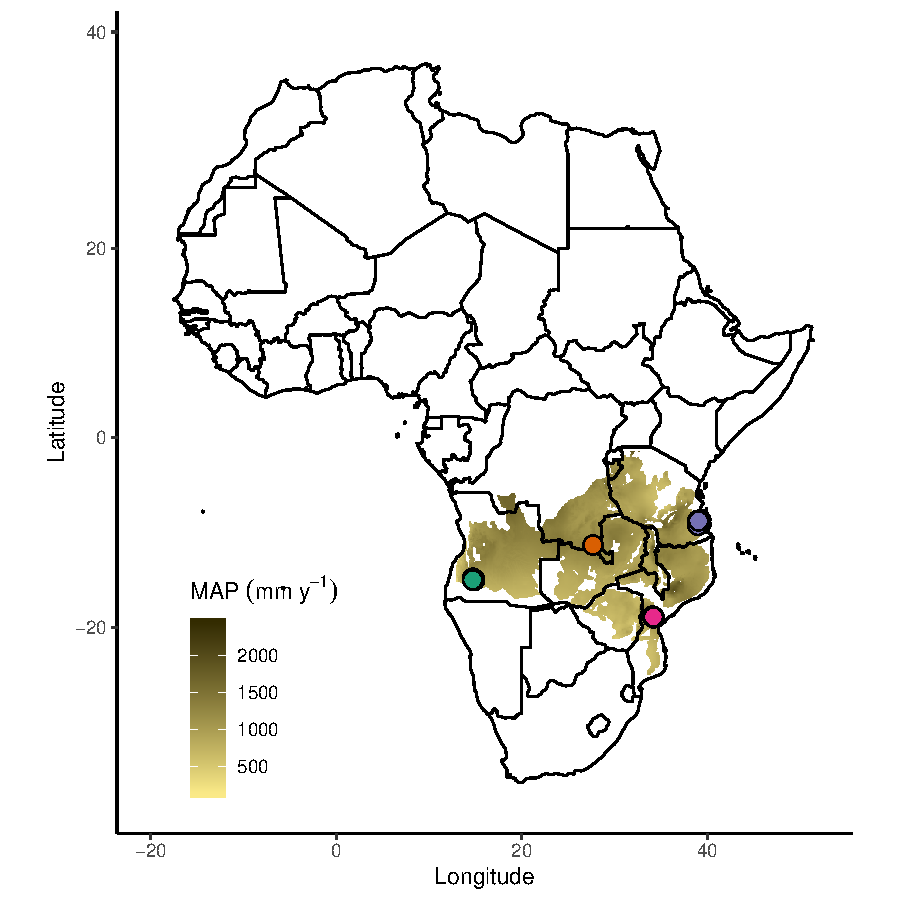
\includegraphics[width=0.475\textwidth]{img/plot_map}}\label{plot_map}}%
    \qquad
\subfloat[]{{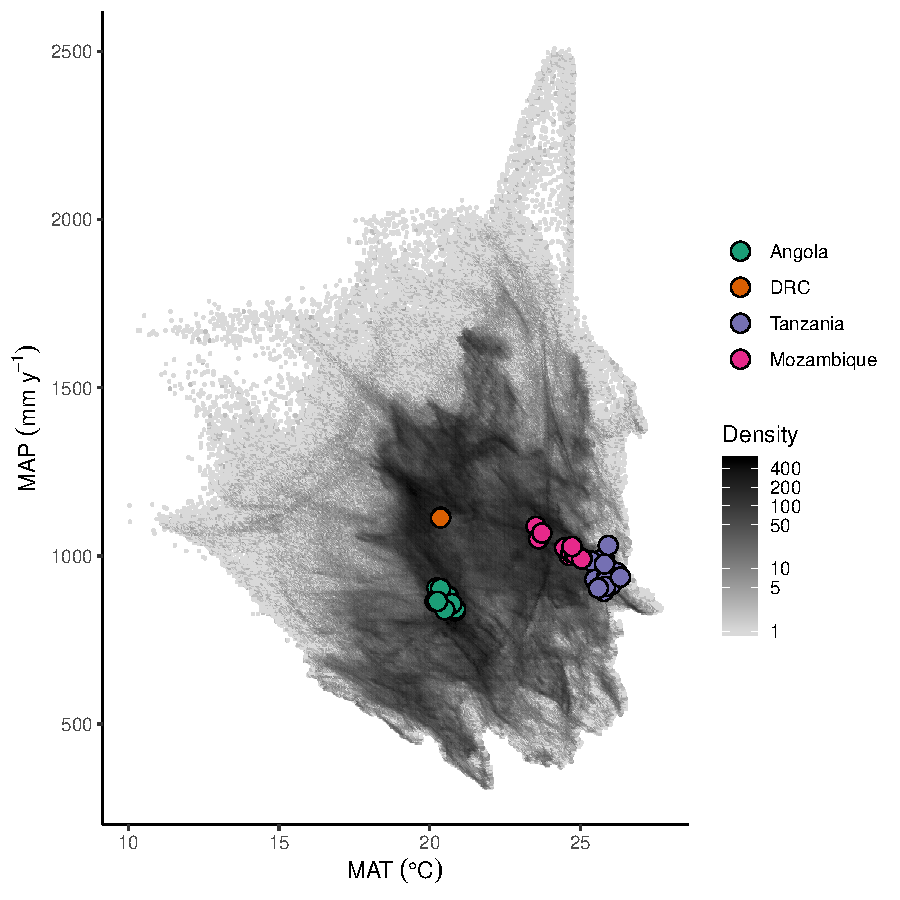
\includegraphics[width=0.475\textwidth]{img/temp_precip}}\label{temp_precip}}%
\caption{Locations of plots used in this study, by (a) geographic location with respect to the distribution of miombo woodland vegetation (shaded brown according to mean annual precipitation) \citep{White1983}, and (b) showing the plot locations compared to the climate space of the miombo ecoregion estimated using the WorldClim dataset over the Miombo woodland vegetation extent with a pixel size of 30 arc seconds (0.86 km\textsuperscript{2} at the equator) \citep{Fick2017}. Note that the density colour scale is log-transformed for visual clarity.}
\end{figure}



% Table created by stargazer v.5.2.2 by Marek Hlavac, Harvard University. E-mail: hlavac at fas.harvard.edu
% Date and time: Fri, Mar 27, 2020 - 14:39:35
\begin{table}[!htbp] \centering 
  \caption{} 
  \label{group_descrip} 
\begin{tabular}{@{\extracolsep{5pt}} cccccccc} 
\\[-1.8ex]\hline 
\hline \\[-1.8ex] 
group & mat & map & cwd & dec\_latitude & dec\_longitude & n\_plots & sp \\ 
\hline \\[-1.8ex] 
Angola & 20.5 & 864 & -815 & -15.12 & 14.81 & 15 & 49 \\ 
DRC & 20.4 & 1115 & -762 & -11.49 & 27.67 & 12 & 89 \\ 
Mozambique & 24.4 & 1029 & -662 & -18.95 & 34.16 & 15 & 162 \\ 
Tanzania & 25.8 & 956 & -754 & -9.05 & 39.05 & 22 & 248 \\ 
\hline \\[-1.8ex] 
\end{tabular} 
\end{table} 


Bicuar National Park covers an area of \textasciitilde{}7900 km\textsuperscript{2}, established as a hunting reserve in 1938, and later as a national park in 1964 (\autoref{bicuar_map}). While fauna populations in the Park were severely damaged by the Angolan civil war, the interior of the Park remains as a largely intact mosaic of miombo woodland, Baikiaea-Burkea woodland, shrub/thicket vegetation and seasonally flooded grassland. Encroachment of agriculture and grazing, particularly along the northwest and western boundaries of the Park, has led to a fragmented park boundary with patches of diminished thicket and woodland in areas of previously farmed land that have been protected since park boundaries were re-established following the end of the civil war.

\rnew{Plots in Tanzania were located predominantly within or near the Mtarure Forest Reserve, administrated by the Tanzania Forest Service and protected from human incursion since their installation. Plots were established between 2010 and 2011 in grassy savanna/woodland areas, with plots located along the road network with a 1 km buffer from the road. Plots in Mozambique were established in 2004, in areas of miombo woodland that had been previously used for agriculture but since left fallow, and areas of undisturbed miombo woodland, located along the road network, with all plots >250 m from the road. Plots in DRC were established in 2009 and located within a larger 800 ha miombo woodland reserve, which consists of undisturbed miombo woodlands. All plots were located quasi-randomly, with consideration to accessibility for future woodland censuses.}

\subsection{Plot data collection}

We sampled \nplotsbicuar{} one hectare plots in Bicuar National Park and collated data from a total of \nplots{} one hectare plots across the miombo ecoregion within four sites. \hyperref[plot_map]{Figure 1a} and \autoref{group_descrip} show the locations and general description of each site, respectively. Plots in Bicuar were situated at least 500 m from the edge of a woodland patch to prevent edge effects which may have altered tree species composition.

Within each plot, every tree stem $\ge$5 cm stem diameter was recorded, except in the DRC plots, where only stems $\ge$10 cm stem diameter were recorded. For each tree stem the species and stem diameter were recorded. Tree species were identified using local botanists at each site and taxonomy was later checked against the African Plant Database \citep{APD2020}. \rchange{In all sites Palgrave and various other texts were used as a guide for species identification in the field}{At all sites, we used \citet{Palgrave2003}, along with other texts, to identify tree species}. Specimens that could not be identified in the field, or subsequently at herbaria, were described as morphospecies. All tree species within the Bicuar National Park plots were identified. Tree coppicing due to fire, herbivory, and human actions is common in miombo woodlands, therefore, for trees with multiple stems, each stem $\ge$5 cm stem diameter was recorded, while the parent tree was also recorded for diversity analyses described below.   

Stem diameter was recorded at 1.3 m from the ground along the stem (diameter at breast height, DBH) as per convention using a diameter tape measure \citep{Kershaw2017}. Where stem abnormalities were present at 1.3 m from the ground, which precluded the accurate estimation of stem diameter at 1.3 m, the stem diameter was recorded at the nearest 10 cm increment above 1.3 m without significant stem abnormalities \citep{Kershaw2017}. To ensure consistency among stem diameter values recorded at different heights, when the stem diameter was recorded at a height other than 1.3 m the stem diameter at 1.3 m was estimated from the recorded stem diameter using a cubic polynomial equation which adjusts for tree stem taper. This equation was calibrated on 100 stems measured at multiple heights in Niassa Province, Mozambique (\hyperref[appendixa]{Appendix A}). Stems below 10 cm stem diameter were not measured in the DRC plots. We therefore estimated the number of 5-10 cm stems in each these plots by extrapolating a linear regression of log stem abundance across the available stem diameter classes.

In addition to the one hectare plots across the miombo ecoregion, we compared the tree biodiversity of undisturbed areas of miombo woodland in Bicuar National Park with areas of disturbed woodland around the edge of the Park that had been previously farmed via shifting cultivation methods, and had since been abandoned and reclaimed within the Park boundaries \autoref{bicuar_map}. We identified areas previously farmed with the help of park rangers and local residents who identified these areas from memory. We conducted \ndegradplots{} plot surveys of woodland diversity and structure in these areas with 20x50 m (0.1 ha) plots, and compared their diversity and structure with 20x50 m subsamples of the \nplotsbicuar{} one hectare plots within the Park interior. Like the one hectare plots, within these smaller 20x50 m plots we recorded the species and stem diameter of every tree stem $\ge$5 cm stem diameter.

\begin{figure}[H]
\centering
	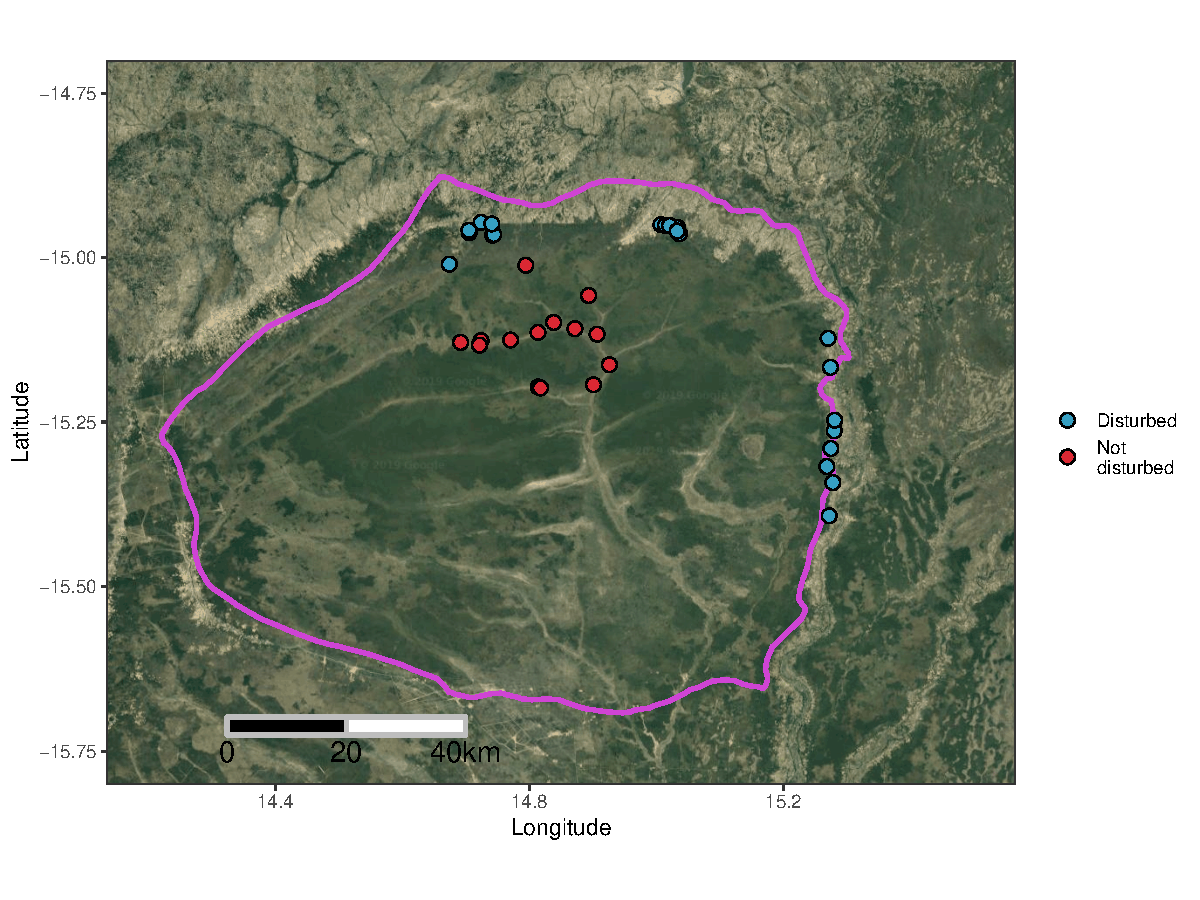
\includegraphics[width=\textwidth]{img/bicuar_map}
	\caption{Location of plots in Bicuar National Park, southwest Angola. The Park boundary is shown as a pink outline, according to \citet{WDPA2019}. One hectare undisturbed plots are shown as red points, while disturbed 20x50 m (0.1 hectare) plots are shown as blue points. The map background is a true colour composite satellite image generated using the Google Maps Static Maps API in the \texttt{ggmap} R package \citep{ggmap}.}
	\label{bicuar_map}
\end{figure}

\subsection{Climatic data}

The WorldClim dataset \citep{Fick2017} was used to gather data on plot-level climatic conditions. We estimated Mean Annual Precipitation (MAP) as the mean of total annual precipitation values between 1970 and 2000, and Mean Annual Temperature (MAT) as the mean of mean annual temperatures between 1970 and 2000. The seasonality of temperature (MAT SD) was calculated as the standard deviation of monthly temperature per year, respectively. We estimated Climatic Water Deficit (CWD) for each plot according to \citep{Chave2014}, as the sum of the difference between monthly rainfall and monthly evapotranspiration when the difference is negative, using the dataset available at \url{http://ups-tlse.fr/pantropical_allometry.htm}, which uses data from the WorldClim dataset 1970-2000.

\subsection{Data analysis}

We calculated the basal area of each stem ($g_{i}$) using:

\begin{equation}
	g_{i} = \pi{} \times (d_{i} / 2)^{2}
\end{equation}

Where $d_{i}$ is the estimated stem diameter of stem $i$ at 1.3 m having accounted for tree taper. We then calculated the total basal area of each plot as the sum of each stem's basal area. For the DRC plots which lacked 5-10 cm stems, we estimated basal area in this stem diameter class from our extrapolation of stem abundance in the 5-10 cm diameter class, assuming a mean stem diameter of 7.5 cm.

All diversity measures were calculated on individual tree-level data, rather than stem-level data, to avoid artificial inflation of abundance for those species which readily coppice. We calculated the alpha diversity of each plot using \rnew{both the tree species richness of trees with stems $\ge$5 cm diameter}, and the Shannon-Wiener index ($H'$) \rnew{(\autoref{shannon})}, using the \texttt{vegan} package in R \citep{vegan}:

\rnew{
\begin{equation}
	H' = -\sum^{S}_{i=1} p_{i} \ln{p_{i}}
	\label{shannon}
\end{equation}
}

\rnew{Where $S$ is the total number of species in the plot, $p_{i}$ is the proportional abundance of the $i$th species and $\ln$ is the natural logarithm.}

We calculated the pairwise beta diversity among sites using the S\o{}rensen coefficient ($S_{S}$) \rnew{(\autoref{sorensen})} 
\citep{Koleff2003}:

\rnew{
\begin{equation}
	\label{sorensen}
	S_S = \frac{2a}{2a + b + c}
\end{equation}
}

\rnew{Where $a$ is the number of species shared between two sites, $b$ is the number of species unique to site 1 and $c$ is the number of species unique to site 2. We calculated $S_{S}$ for each pairwise combination of sites using aggregated species composition data from all plots in each site. The value of $S_{S}$, which ranges between zero and one, was multiplied by 100 to give a ``percentage similarity'' between communities in species composition.}

We estimated abundance evenness for each plot using the Shannon equitability index ($E_{H'}$) \citep{Smith1996} which is the ratio of $H'$ to the log transformed species richness.

We analysed the difference in alpha diversity measures and woodland structural variables among groups of plots using Analysis of Variance (ANOVA) statistical models, with a null hypothesis that there was no difference among the mean values of groups of plots. Post-hoc Tukey's HSD tests were used to investigate the degree to which pairwise combinations of plot groups differed in each case.

We used Non-metric Multidimensional Scaling (NMDS) to assess the variation in species composition among one hectare plots, and also between disturbed and undisturbed 20x50 m plots within Bicuar National Park, using the \texttt{vegan} R package. The number of dimensions for NMDS was minimised while ensuring the stress value of the NMDS fit was $\le$0.1. NMDS analyses were run with 500 random restarts to ensure a global solution was reached. We used Bray-Curtis dissimilarity as the optimal measure of ecological distance \citep{Legendre2013}. We fit plot-level estimates of MAP, MAT, the seasonality of MAT and CWD to the first two axes of the resulting ordination using the \texttt{envfit} function in the \texttt{vegan} R package to investigate how these environmental factors influenced the grouping of species composition among plots. All analyses were conducted in R version 3.6.1 \citep{RCoreTeam2019}.

% Materials and Methods should be described with sufficient details to allow others to replicate and build on published results. Please note that publication of your manuscript implicates that you must make all materials, data, computer code, and protocols associated with the publication available to readers. Please disclose at the submission stage any restrictions on the availability of materials or information. New methods and protocols should be described in detail while well-established methods can be briefly described and appropriately cited.
% Research manuscripts reporting large datasets that are deposited in a publicly available database should specify where the data have been deposited and provide the relevant accession numbers. If the accession numbers have not yet been obtained at the time of submission, please state that they will be provided during review. They must be provided prior to publication.

%%%%%%%%%%%%%%%%%%%%%%%%%%%%%%%%%%%%%%%%%%
\section{Results}

\subsection{Alpha diversity}

In Bicuar National Park we measured a total of \nbicuartrees{} trees within the one hectare plots, and across the four sites,  a total of \ntrees{} trees were sampled. Trees in Bicuar National Park belonged to \nbicuarspecies{} species within \nbicuarfamilies{} families. Across all four sites we recorded \nspecies{} species from \nfamilies{} families. The most diverse family within each site and among all plots was Fabaceae with \nfabaceaespecies{} species. We encountered \nbicuaruniquespecies{} tree species in Bicuar National Park which were not found in the other miombo woodland plots (\autoref{bicuar_species}). The most common of these unique species were \textit{Brachystegia tamarindoides} (n = \nbg{}), \textit{Baikiaea plurijuga} (n = \nbp{}) and \textit{Baphia massaiensis} (n = \nbm{}). Four species unique to Bicuar National Park within this dataset only had one individual recorded: \textit{Elachyptera parvifolia}, \textit{Entandrophragma spicatum}, \textit{Oldfieldia dactylophylla}, \textit{Peltophorum africanum}.


% Table created by stargazer v.5.2.2 by Marek Hlavac, Harvard University. E-mail: hlavac at fas.harvard.edu
% Date and time: Thu, Jan 30, 2020 - 11:46:11
\begin{table}[!htbp] \centering 
  \caption{} 
  \label{bicuar_species} 
\begin{tabular}{@{\extracolsep{5pt}} cccccc} 
\\[-1.8ex]\hline 
\hline \\[-1.8ex] 
family & species\_binomial & dbh & basal\_area & total\_freq & mean\_freq \\ 
\hline \\[-1.8ex] 
Fabaceae & Albizia antunesiana & 9.1(2.03) & 0.07(0.040) & 40 & 8(4.81) \\ 
Fabaceae & \textbackslash textbf\{\textasteriskcentered Baikiaea plurijuga\} & 28.9(0.75) & 1.72(0.570) & 331 & 55.2(17.83) \\ 
Fabaceae & \textbackslash textbf\{\textasteriskcentered Baphia bequaertii\} & 7.4(0.36) & 0.08(0.050) & 127 & 31.8(18.14) \\ 
Fabaceae & \textbackslash textbf\{\textasteriskcentered Baphia massaiensis\} & 6.6(0.17) & 0.05(0.020) & 303 & 30.3(11.20) \\ 
Fabaceae & Bobgunnia madagascariensis & 7.8(0.91) & 0.04(0.020) & 32 & 10.7(9.67) \\ 
Fabaceae & \textbackslash textbf\{\textasteriskcentered Brachystegia glaucescens\} & 12.9(0.48) & 1.14(0.430) & 576 & 115.2(72.67) \\ 
Fabaceae & Brachystegia spiciformis & 11.4(0.52) & 0.74(0.430) & 326 & 81.5(46.56) \\ 
Phyllanthaceae & \textbackslash textbf\{\textasteriskcentered Bridelia mollis\} & 5.7(0.31) & 0.02(NA) & 23 & 23(NA) \\ 
Fabaceae & Burkea africana & 8.5(0.33) & 0.39(0.120) & 863 & 71.9(19.11) \\ 
Combretaceae & Combretum apiculatum & 7.6(0.45) & 0.06(0.040) & 60 & 30(15.00) \\ 
Combretaceae & Combretum celastroides & 5.6(0.34) & \textless 0.01(0.000) & 7 & 3.5(2.50) \\ 
Combretaceae & Combretum collinum & 6.3(0.09) & 0.07(0.020) & 609 & 50.8(20.48) \\ 
Combretaceae & \textbackslash textbf\{\textasteriskcentered Combretum hereroense\} & 6.7(0.26) & 0.02(0.010) & 73 & 12.2(5.69) \\ 
Combretaceae & \textbackslash textbf\{\textasteriskcentered Combretum psidioides\} & 7.4(0.43) & 0.01(0.010) & 33 & 6.6(4.17) \\ 
Combretaceae & Combretum zeyheri & 6.3(0.35) & 0.01(0.000) & 61 & 10.2(3.03) \\ 
Euphorbiaceae & \textbackslash textbf\{\textasteriskcentered Croton gratissimus\} & 6.1(1.55) & \textless 0.01(NA) & 4 & 4(NA) \\ 
Ebenaceae & \textbackslash textbf\{\textasteriskcentered Diospyros batocana\} & 8.4(2.14) & \textless 0.01(0.000) & 2 & 1(0.00) \\ 
Ebenaceae & \textbackslash textbf\{\textasteriskcentered Diospyros kirkii\} & 9.3(1.64) & 0.03(NA) & 11 & 11(NA) \\ 
Apocynaceae & Diplorhynchus condylocarpon & 8.2(0.52) & 0.08(0.060) & 174 & 19.3(7.57) \\ 
Malvaceae & \textbackslash textbf\{\textasteriskcentered Dombeya rotundifolia\} & 5.5(0.19) & \textless 0.01(NA) & 2 & 2(NA) \\ 
Celastraceae & \textbackslash textbf\{\textasteriskcentered Elachyptera parvifolia\} & 7.3(NA) & \textless 0.01(NA) & 1 & 1(NA) \\ 
Meliaceae & \textbackslash textbf\{\textasteriskcentered Entandrophragma spicatum\} & 14.6(NA) & \textless 0.01(NA) & 1 & 1(NA) \\ 
Fabaceae & Erythrophleum africanum & 9.0(0.84) & 0.10(0.040) & 128 & 18.3(6.82) \\ 
Rubiaceae & \textbackslash textbf\{\textasteriskcentered Gardenia volkensii\} & 5.6(1.15) & \textless 0.01(0.000) & 5 & 2.5(1.50) \\ 
Fabaceae & \textbackslash textbf\{\textasteriskcentered Guibourtia coleosperma\} & 7.2(1.00) & 0.02(0.010) & 31 & 6.2(3.54) \\ 
Phyllanthaceae & Hymenocardia acida & 5.9(1.25) & \textless 0.01(NA) & 6 & 6(NA) \\ 
Fabaceae & Julbernardia paniculata & 10.1(0.21) & 0.92(0.200) & 1624 & 162.4(50.60) \\ 
Fabaceae & \textbackslash textbf\{\textasteriskcentered Lonchocarpus nelsii\} & 13.4(0.88) & 0.15(0.030) & 165 & 15(2.77) \\ 
Dipterocarpaceae & \textbackslash textbf\{\textasteriskcentered Monotes angolensis\} & 7.4(0.83) & \textless 0.01(0.000) & 2 & 1(0.00) \\ 
Ochnaceae & \textbackslash textbf\{\textasteriskcentered Ochna pulchra\} & 6.5(0.80) & 0.01(0.000) & 26 & 8.7(3.76) \\ 
Picrodendraceae & \textbackslash textbf\{\textasteriskcentered Oldfieldia dactylophylla\} & 8.5(NA) & \textless 0.01(NA) & 1 & 1(NA) \\ 
Fabaceae & \textbackslash textbf\{\textasteriskcentered Peltophorum africanum\} & 11.5(NA) & \textless 0.01(NA) & 1 & 1(NA) \\ 
Fabaceae & Pericopsis angolensis & 8.4(0.61) & 0.06(0.020) & 97 & 12.1(5.08) \\ 
Phyllanthaceae & Pseudolachnostylis maprouneifolia & 6.7(0.45) & 0.03(0.010) & 84 & 9.3(3.00) \\ 
Combretaceae & \textbackslash textbf\{\textasteriskcentered Pteleopsis anisoptera\} & 6.8(0.46) & 0.07(0.020) & 81 & 20.2(15.11) \\ 
Fabaceae & Pterocarpus angolensis & 13.0(0.61) & 0.15(0.100) & 102 & 17(8.65) \\ 
Fabaceae & \textbackslash textbf\{\textasteriskcentered Pterocarpus lucens\} & 6.9(0.94) & \textless 0.01(NA) & 4 & 4(NA) \\ 
Rubiaceae & \textbackslash textbf\{\textasteriskcentered Rothmannia engleriana\} & 6.8(0.66) & \textless 0.01(0.000) & 5 & 1.7(0.67) \\ 
Euphorbiaceae & \textbackslash textbf\{\textasteriskcentered Schinziophyton rautanenii\} & 8.0(2.82) & \textless 0.01(NA) & 3 & 3(NA) \\ 
Polygalaceae & Securidaca longepedunculata & 7.3(1.12) & \textless 0.01(0.010) & 4 & 2(1.00) \\ 
Loganiaceae & Strychnos cocculoides & 10.4(1.17) & 0.03(0.020) & 19 & 6.3(3.53) \\ 
Loganiaceae & \textbackslash textbf\{\textasteriskcentered Strychnos pungens\} & 6.1(0.48) & \textless 0.01(0.000) & 18 & 3.6(0.93) \\ 
Loganiaceae & Strychnos spinosa & 6.8(0.36) & 0.02(0.010) & 97 & 9.7(4.07) \\ 
Combretaceae & \textbackslash textbf\{\textasteriskcentered Terminalia brachystemma\} & 6.5(0.21) & 0.04(0.020) & 174 & 29(12.04) \\ 
Combretaceae & Terminalia sericea & 7.1(0.28) & 0.06(0.030) & 214 & 23.8(12.18) \\ 
Ximeniaceae & Ximenia americana & 6.1(0.53) & \textless 0.01(0.000) & 7 & 1.8(0.25) \\ 
Sapindaceae & Zanha africana & 9.4(1.12) & 0.01(NA) & 6 & 6(NA) \\ 
Rhamnaceae & \textbackslash textbf\{\textasteriskcentered Ziziphus abyssinica\} & 5.9(1.13) & \textless 0.01(NA) & 2 & 2(NA) \\ 
\hline \\[-1.8ex] 
\end{tabular} 
\end{table} 


Alpha diversity in Bicuar National Park was low compared to other sites (\autoref{div_box}). Mean $H'$ across plots in Bicuar National Park was \bicuarshannon{}. An ANOVA showed a significant difference in $H'$ among sites (\lmshannon{}, \autoref{anova_table}), and a post-hoc Tukey's test showed that $H'$ in plots in Bicuar National Park was significantly different from those in DRC ($H'$ = \drcshannon{}, \tukeyshannonbicuardrc{}), Mozambique ($H'$ = \nhamshannon{}, \tukeyshannonbicuarnham{}) and Tanzania ($H'$ = \kilwashannon{}, \tukeyshannonbicuarkilwa{}). Variation in $H'$ is large within Bicuar National Park, with $H'$ ranging from \bicuarminshannon{} to \bicuarmaxshannon{}, but this was a similar range to other sites. In contrast, the range of species richness within Bicuar National Park was much lower than other sites, suggesting that the wide range in $H'$ was caused by variation in abundance evenness.

\begin{figure}[H]
\centering
	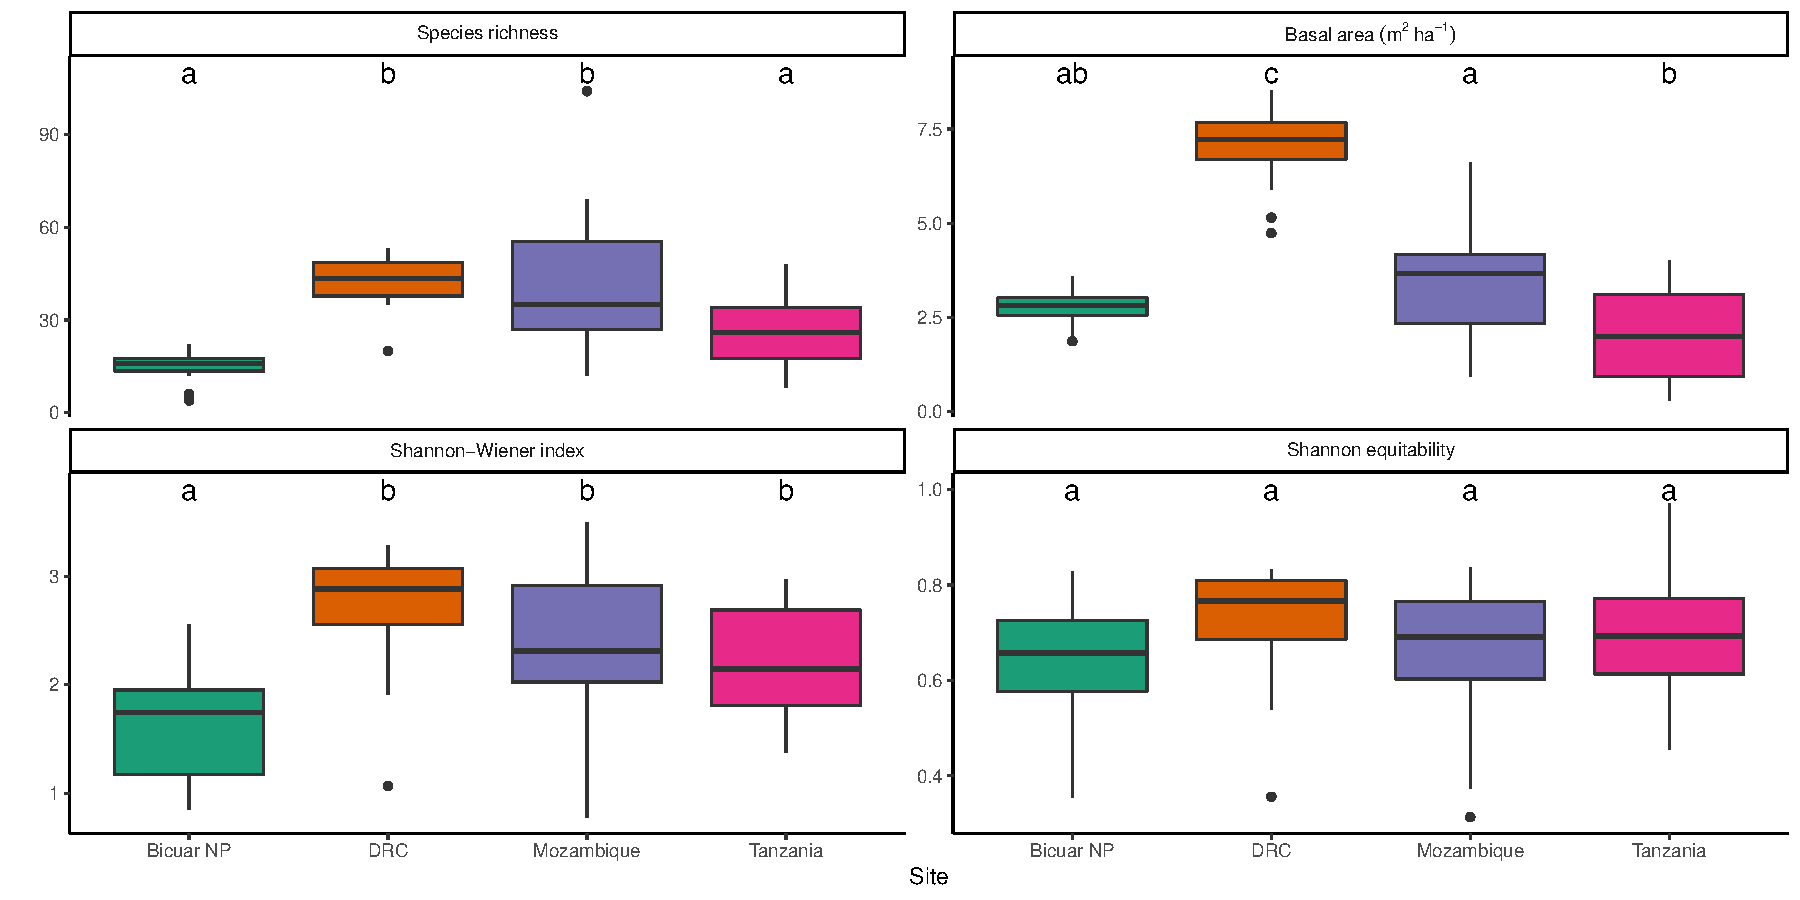
\includegraphics[width=\textwidth]{img/div_box}
	\caption{Variation of alpha diversity estimates and basal area among sites. Boxes bound the 1st and 3rd quartiles, with the median within the box. Whiskers represent 1.5 times the interquartile range plus or minus the 1st and 3rd quartiles, respectively. Values found beyond the whiskers are shown individually as points. \rnew{Letter labels above each box refer to groupings from post-hoc Tukey's tests on the ANOVA of each diversity/structure variable. Sites sharing a letter do not differ significantly (p<0.05)}.}
    \label{div_box}
\end{figure}

\rnew{

% Table created by stargazer v.5.2.2 by Marek Hlavac, Harvard University. E-mail: hlavac at fas.harvard.edu
% Date and time: Fri, Mar 27, 2020 - 14:32:56
\begin{table}[!htbp] \centering 
  \caption{} 
  \label{} 
\begin{tabular}{@{\extracolsep{5pt}}lcccc} 
\\[-1.8ex]\hline 
\hline \\[-1.8ex] 
 & \multicolumn{4}{c}{\textit{Dependent variable:}} \\ 
\cline{2-5} 
\\[-1.8ex] & rich & basal\_area & shannon & shannon\_equit \\ 
\\[-1.8ex] & (1) & (2) & (3) & (4)\\ 
\hline \\[-1.8ex] 
 groupdrc & 27.920$^{***}$ & 4.175$^{***}$ & 1.055$^{***}$ & 0.080 \\ 
  & (5.538) & (0.452) & (0.236) & (0.053) \\ 
  & & & & \\ 
 groupkilwa & 12.440$^{**}$ & $-$0.721$^{*}$ & 0.605$^{***}$ & 0.064 \\ 
  & (4.788) & (0.391) & (0.204) & (0.046) \\ 
  & & & & \\ 
 groupnham & 27.930$^{***}$ & 0.653 & 0.792$^{***}$ & 0.028 \\ 
  & (5.221) & (0.427) & (0.223) & (0.050) \\ 
  & & & & \\ 
 Constant & 14.330$^{***}$ & 2.778$^{***}$ & 1.617$^{***}$ & 0.631$^{***}$ \\ 
  & (3.692) & (0.302) & (0.158) & (0.035) \\ 
  & & & & \\ 
\hline \\[-1.8ex] 
Observations & 64 & 64 & 64 & 64 \\ 
R$^{2}$ & 0.394 & 0.706 & 0.274 & 0.048 \\ 
Adjusted R$^{2}$ & 0.363 & 0.691 & 0.237 & $-$0.00000 \\ 
Residual Std. Error (df = 60) & 14.300 & 1.168 & 0.611 & 0.137 \\ 
F Statistic (df = 3; 60) & 12.980$^{***}$ & 48.040$^{***}$ & 7.537$^{***}$ & 1.000 \\ 
\hline 
\hline \\[-1.8ex] 
\multicolumn{5}{r}{$^{*}$p$<$0.1; $^{**}$p$<$0.05; $^{***}$p$<$0.01} \\ 
\end{tabular} 
\end{table} 

}

\subsection{Beta diversity}

The NMDS of plot species composition among one hectare plots was run with four dimensions. The stress value was \nmdsstress{}. Plot diversity in Bicuar National Park formed three distinct groups within axes 1 and 2 of the NMDS ordination. Bicuar plots 9, 13, and 15 were characterised by high abundances of \textit{Baikiaea plurijuga}, \textit{Baphia massaiensis} and \textit{Croton gratissimus}, according to species scores from the NMDS. Bicuar plots 4, 11, and 12 were characterised  by \textit{Brachystegia tamarindoides}, and \textit{Ochna pulchra}. The third group consisting of the remaining seven plots surprisingly had a species composition most similar to that of plots in the DRC group according to the NMDS, sharing the core miombo species of \textit{Julbernardia paniculata} and \textit{Pterocarpus angolensis}. This group of plots in Bicuar National Park was further characterised by the abundance of \textit{Pterocarpus lucens}, \textit{Strychnos pungens} and \textit{Bridelia mollis} however, which were not present in the DRC plots. All environmental factors fitted to the NMDS ordination correlated significantly with the grouping of plots (\hyperref[all_nmds_envfit]{Figure 4a}). MAT explained the most variation in plot position on the first two NMDS axes (\nmdsmat{}), followed by CWD (\nmdsmapsd{}), the seasonality of MAT (\nmdsmatsd{}) and MAP (\nmdsmap{}). Variation in MAP explained much of the difference among plots in Bicuar National Park versus those in Tanzania and Mozambique. Axes 3 and 4 showed a greater degree of overlap in species composition among plot groups, with plots from Bicuar National Park similar to a select few plots in both Tanzania and Mozambique (\hyperref[all_nmds_envfit_low]{Figure 4b}). Axis 3 distinguished plots in Bicuar NP from those in DRC, while plots from all geographic area overlapped in their distribution across Axis 4. Axes 3 and 4 largely reflected distribution patterns of less abundant species and not the dominant species in the vegetation.


\begin{figure}[H]
	\centering
	\subfloat[]{{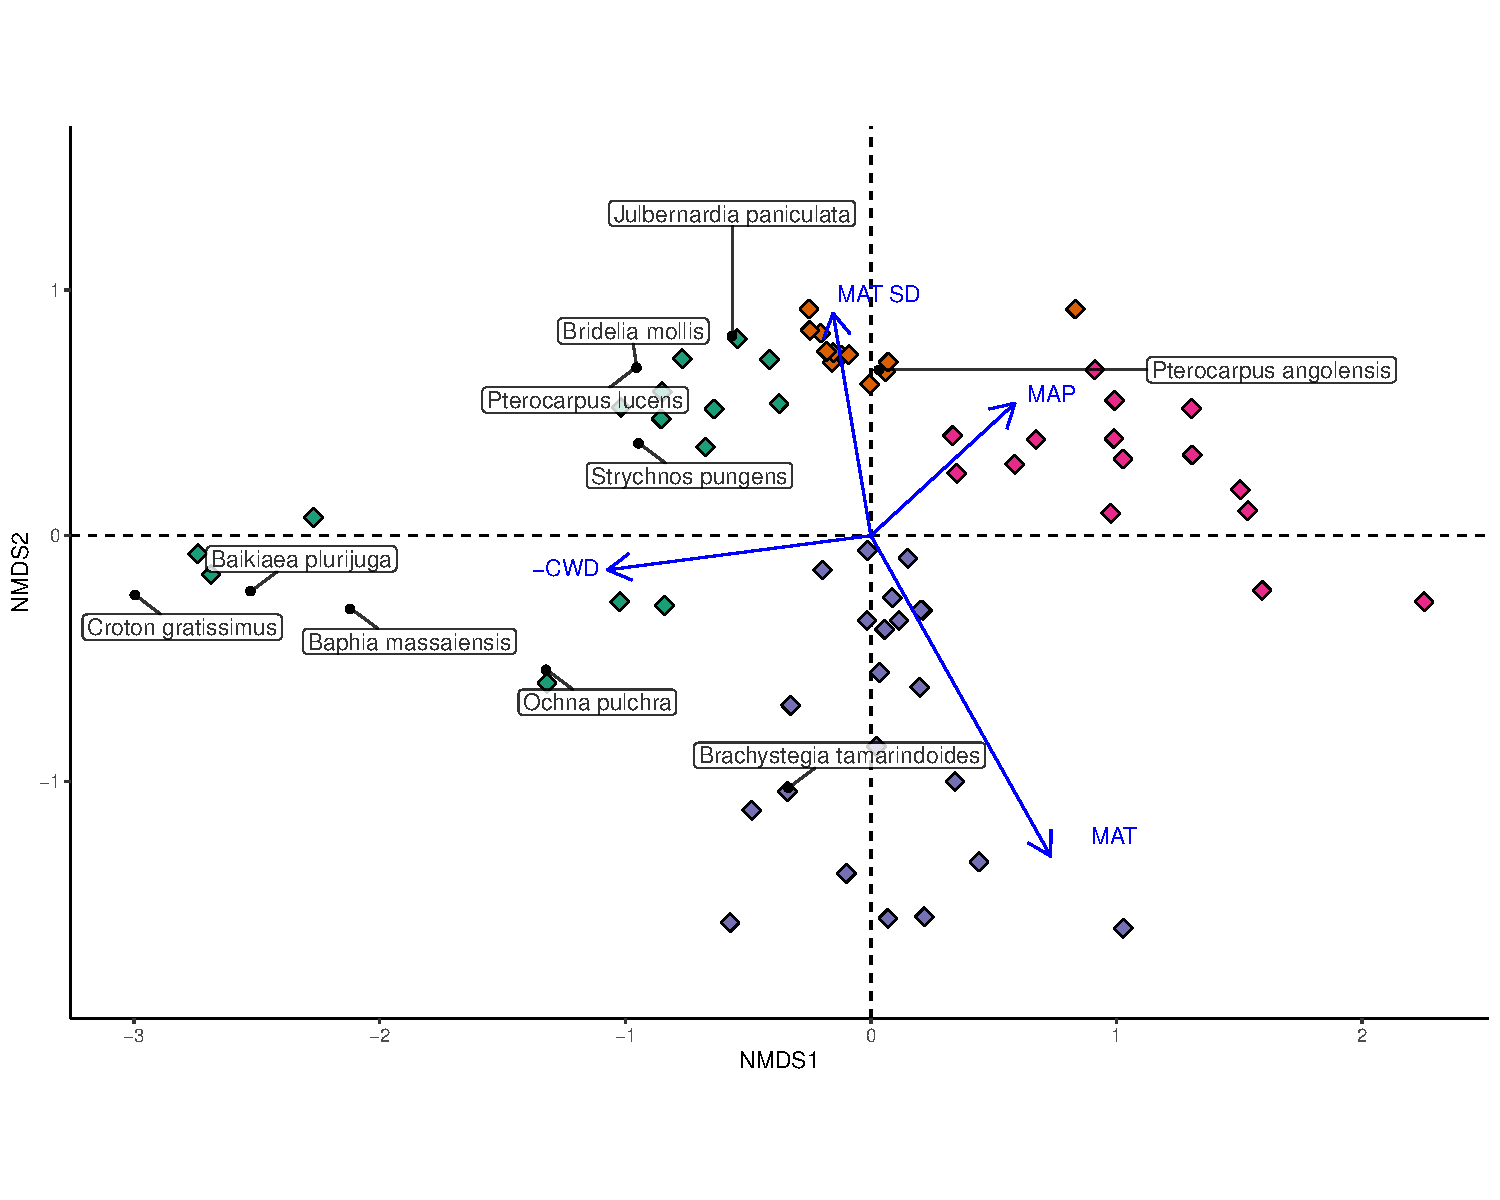
\includegraphics[width=0.475\textwidth]{img/all_nmds_envfit}}\label{all_nmds_envfit}}%
    \qquad
\subfloat[]{{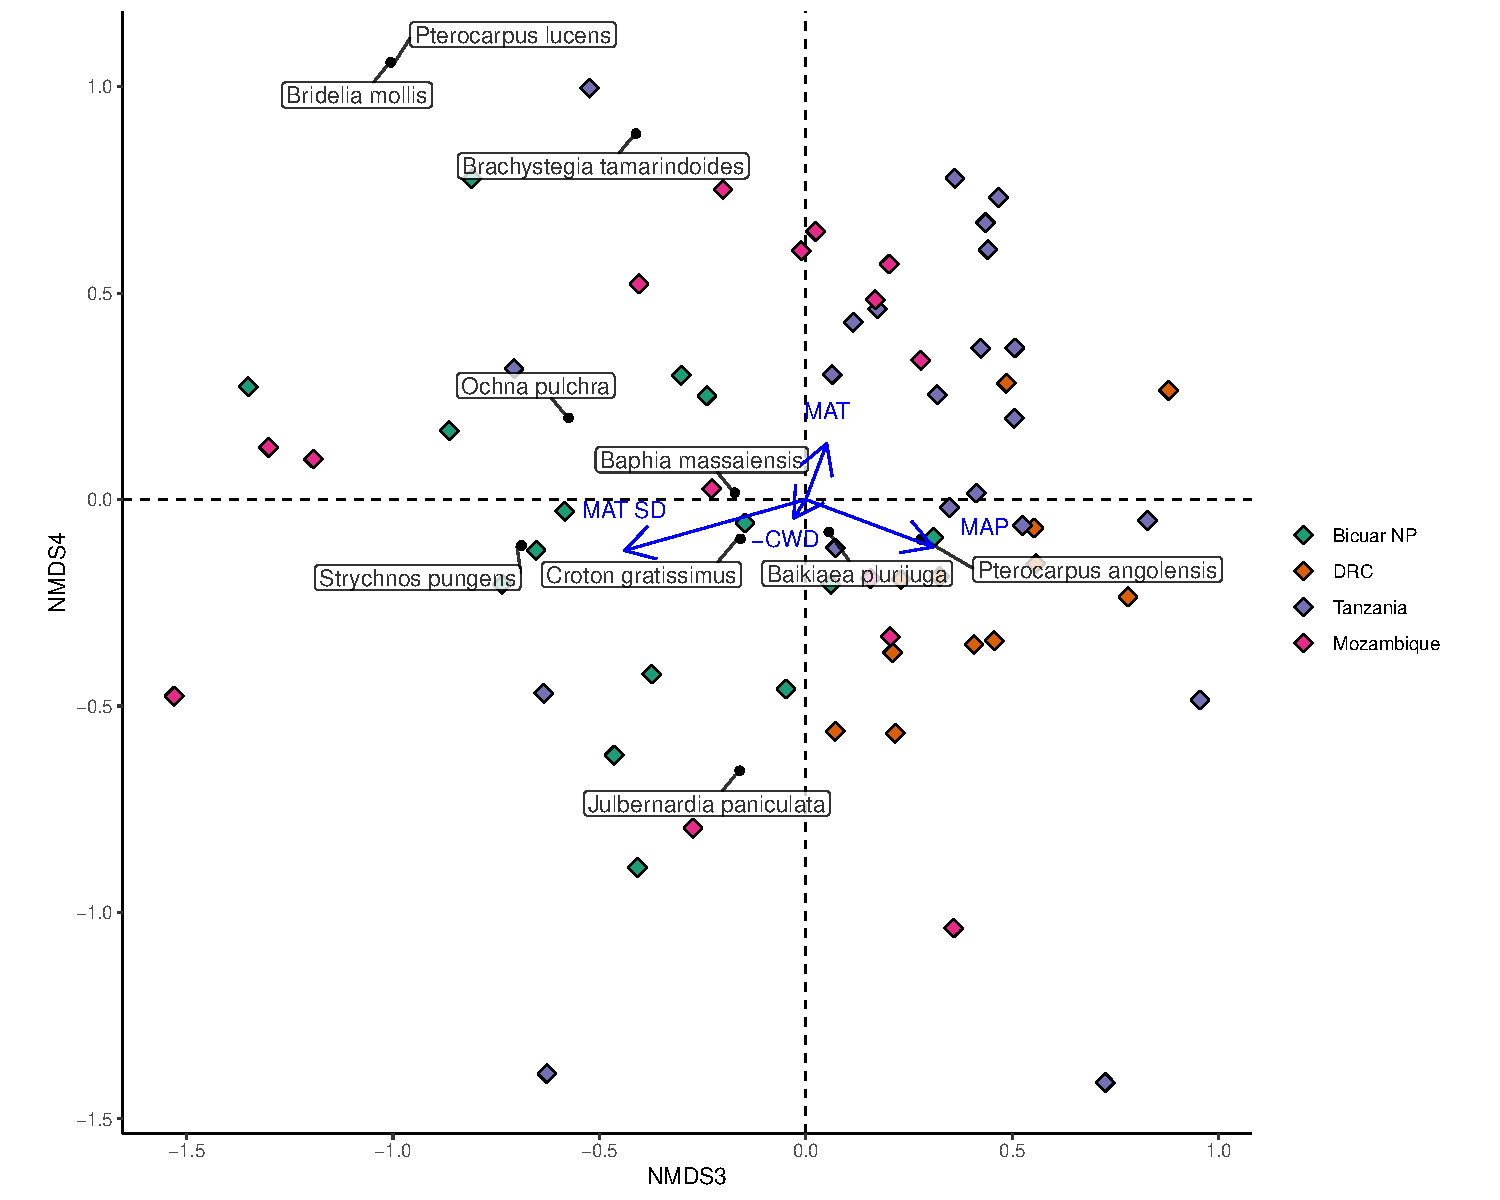
\includegraphics[width=0.475\textwidth]{img/all_nmds_envfit_low}}\label{all_nmds_envfit_low}}%
\caption{Environmental factors fitted to axes 1 and 2 (a), 3 and 4 (b) of the NMDS ordination of species composition of one hectare plots, showing the variation in plot species composition within and among sites. Diamonds are plot scores coloured by site. The lengths of arrows indicating environmental factor fits to the first two ordination axes are scaled by R\textsuperscript{2}. Arrows point in the direction of increasing values of that environmental factor. Note that Climatic Water Deficit (CWD) is expressed in more intuitively as the negative inverse of CWD, thus larger values indicate higher levels of CWD.}
\end{figure}

The pairwise S\o{}rensen coefficient of percentage similarity ($S_{S}$) showed that the species composition of plots in Bicuar National Park had low similarity with other sites in the study, sharing few species with other sites (\autoref{site_pairs_js}). Similar to the NMDS, these results show that plots in Bicuar National Park are most similar to those found in DRC. 


% Table created by stargazer v.5.2.2 by Marek Hlavac, Harvard University. E-mail: hlavac at fas.harvard.edu
% Date and time: Tue, Jan 28, 2020 - 14:16:40
\begin{table}[!htbp] \centering 
  \caption{} 
  \label{site_pairs_js} 
\begin{tabular}{@{\extracolsep{5pt}} cccc} 
\\[-1.8ex]\hline 
\hline \\[-1.8ex] 
col1 & col2 & js & sp\_share \\ 
\hline \\[-1.8ex] 
bicuar(34) & drc(74) & 20.6 & $14$ \\ 
bicuar(34) & kilwa(147) & 13.4 & $14$ \\ 
bicuar(37) & nham(236) & 7.5 & $11$ \\ 
drc(64) & kilwa(137) & 19.3 & $24$ \\ 
drc(69) & nham(228) & 11.3 & $19$ \\ 
kilwa(139) & nham(225) & 10.8 & $22$ \\ 
\hline \\[-1.8ex] 
\end{tabular} 
\end{table} 


\subsection{Woodland structure}

Mean basal area of plots in Bicuar National Park was \babicuar{} m\textsuperscript{2} ha\textsuperscript{-1}, ranging from \bicuarbamin{} to \bicuarbamax{} m\textsuperscript{2} ha\textsuperscript{-1} (\autoref{div_box}). An ANOVA showed a significant difference in basal area among sites (\lmba{}), and a post-hoc Tukey's test showed that basal area in Bicuar National Park was significantly lower than plots in DRC (BA = \badrc{} m\textsuperscript{2} ha\textsuperscript{-1}, \tukeybabicuardrc{}), but there were no significant differences between Bicuar and Mozambique (BA = \banham{} m\textsuperscript{2} ha\textsuperscript{-1}, \tukeybabicuarnham{}) or Tanzania (BA = \bakilwa{} m\textsuperscript{2} ha\textsuperscript{-1}, \tukeybabicuarkilwa{}) (\autoref{div_box}). Additionally, Bicuar plots had less variation in basal area among plots than other sites. Plots in Bicuar with the highest basal area were dominated by \textit{Baikiaea plurijuga} and \textit{Baphia massaiensis} (Plots 9, 13, and 15). 

The stem diameter abundance distribution in Bicuar National Park was comparable with other sites (\autoref{stem_ab_dbh_bin}), albeit with fewer stems in each class. The slope of log mean stem size distribution among diameter bins was \dbhslopebicuar{} in Bicuar National Park, \dbhslopedrc{} in DRC, \dbhslopekilwa{} in Tanzania, and \dbhslopenham{} in Mozambique.  

\begin{figure}[H]
\centering
	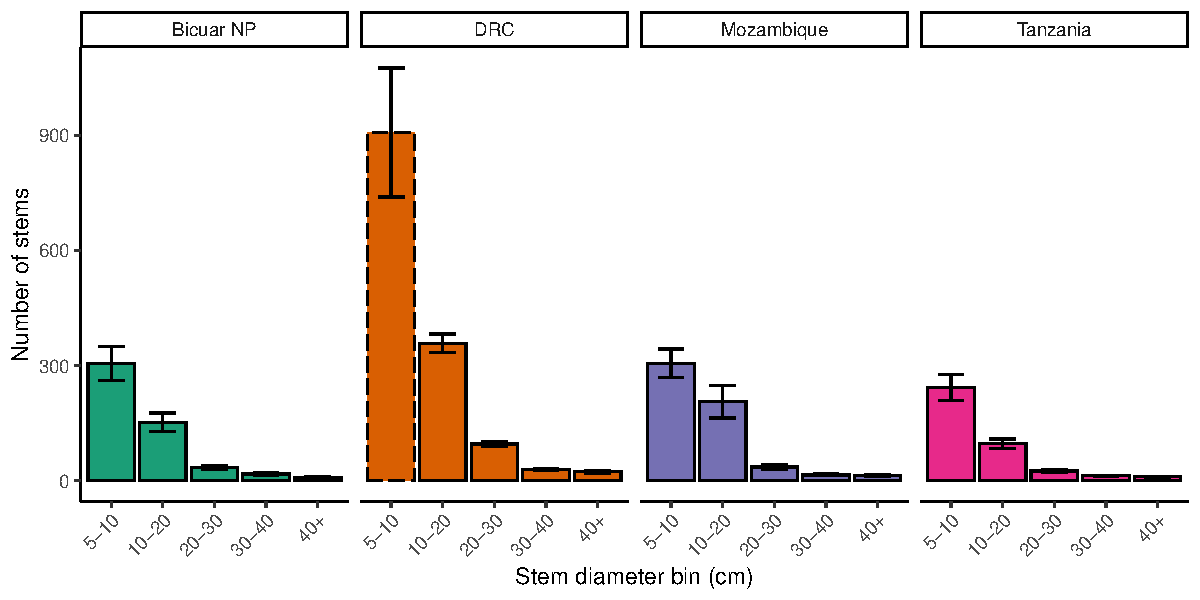
\includegraphics[width=\textwidth]{img/stem_ab_dbh_bin_group}
	\caption{Ranked variation between plots in stem number within each site, with bars according to stem diameter class. Error bars are the mean $\pm$ 1 standard error. The dashed bar for the DRC 5-10 cm stem diameter class indicates that these measurements were estimated by extrapolating a linear regression of log stem abundance across the available stem diameter classes for DRC.}
	\label{stem_ab_dbh_bin}
\end{figure}

\subsection{Effect of disturbance via shifting cultivation on diversity within Bicuar National Park}

There was a clear difference in the species composition of previously farmed disturbed woodland plots and undisturbed woodland plots, but with some overlap (\autoref{bicuar_degrad_nmds}). Notably, Plots 4 and 7 in putatively undisturbed woodland have a species composition more resembling the disturbed plots. These two plots were dominated by \textit{Brachystegia tamarindoides} and \textit{Burkea africana}, with \textit{B. africana} being a species which occurred frequently as a pioneer in the disturbed plots. The undisturbed plots 15, 13, and 9 represent distinct outliers in the NMDS. These three plots were dominated by \textit{Baikiaea plurijuga} which was not encountered in the disturbed plots. The most common species in the disturbed plots was \textit{Baphia massaiensis} (n = \nbmdegrad{}), with a mean stem diameter of \bmdbhdegrad{} cm, while in the undisturbed plots the most common species was \textit{Julbernardia paniculata} (n = \njpdegrad{}), with a mean stem diameter of \jpdbhbicuar{} cm. Mean alpha diversity was marginally higher in disturbed plots ($H'$ = \degradshannon{}) than in undisturbed plots ($H'$ = \bicuarsubshannon{}) and an ANOVA showed that there was a significant difference in $H'$ between the two plot types(\lmshannondegrad{}) (\autoref{degrad_box}, \autoref{degrad_anova_table}). Mean plot species richness was also lower in undisturbed plots (\bicuarsubrich{}) than disturbed plots (\degradrich{}). Mean $E_{H'}$ was \degradequit{} in disturbed plots and \bicuarsubequit{} in undisturbed plots but there was no significant difference between disturbed and undisturbed plots according to an ANOVA (\lmequitdegrad{}). \ndegradonlyspecies{} species were found only in the disturbed plots and not in the undisturbed plots. The most common of these were \textit{Combretum celastroides} (n = \nccdegrad{}), \textit{Acacia reficiens} (n = \nvrdegrad{}), and \textit{Gardenia ternifolia} (n = \ngtdegrad{}). \nbigonlyspecies{} were found only in undisturbed plots, the most common being \textit{Brachystegia spiciformis} (n = \nbsbig{}), \textit{Baikiaea plurijuga} (n = \nbpbig{}) and \textit{Combretum apiculatum} (n = \ncabig{}). Mean basal area was higher in undisturbed plots (\bicuarsubba{} m\textsuperscript{2} ha\textsuperscript{-1}) than disturbed plots (\degradba{} m\textsuperscript{2} ha\textsuperscript{-1}). 

Mean stem density was higher in disturbed plots (\stemdensdegrad{} stems ha\textsuperscript{-1}) than undisturbed plots (\stemdensbicuar{} stems ha\textsuperscript{-1}). The stem diameter abundance distribution in disturbed plots showed that many more stems were from the 5-10 cm diameter class in disturbed plots, while the disturbed plots had fewer stems in the 10-20 cm size class. Both disturbed and undisturbed plots had a similar abundance of stems in larger stem diameter classes (\autoref{degrad_dbh_bin}). Multi-stemmed trees in disturbed plots tended to have a greater number of stems per tree (\multistemdegrad{}) than multi-stemmed trees in undisturbed plots (\multistembicuar{}).

\begin{figure}[H]
\centering
	\includegraphics[width=0.8\textwidth]{img/bicuar_degrad_nmds}
	\caption{NMDS ordination of species composition of 20x50 m (0.1 ha) plots showing plot scores as coloured diamonds located in disturbed (blue) and undisturbed (red) areas of woodland in Bicuar National Park.}
	\label{bicuar_degrad_nmds}
\end{figure}

\begin{figure}[H]
\centering
	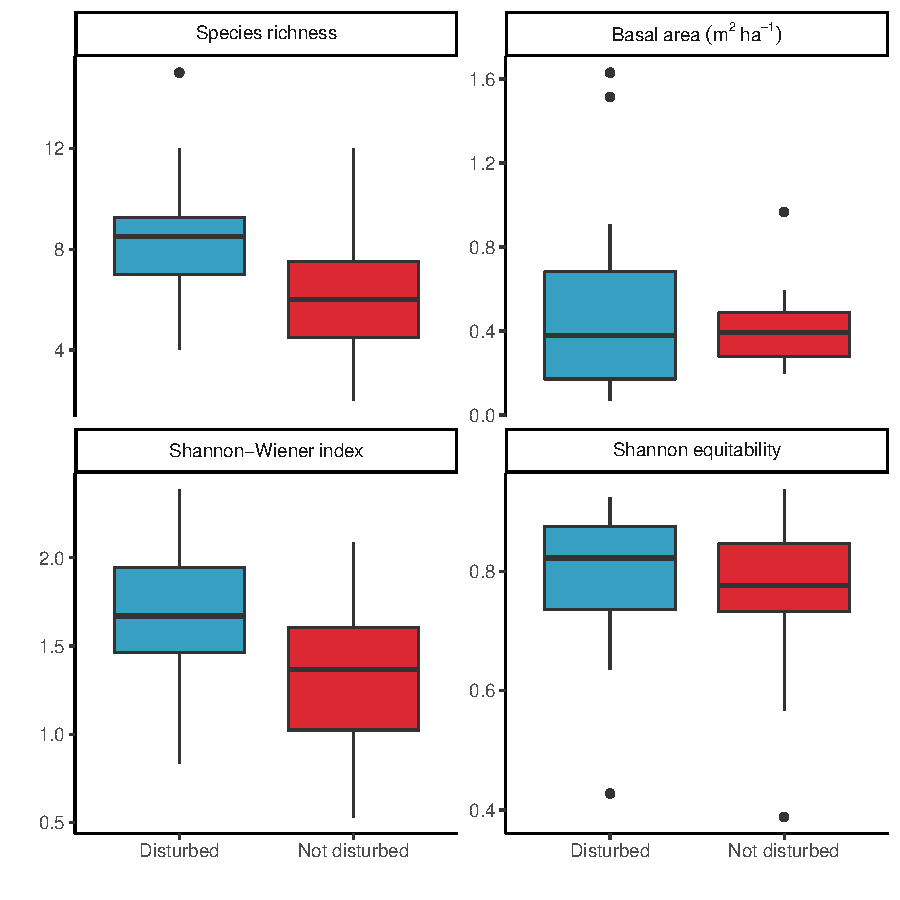
\includegraphics[width=0.8\textwidth]{img/degrad_box}
	\caption{The variation in diversity and woodland structure between disturbed and undisturbed 20x50 m (0.1 ha) plots in Bicuar National Park. Boxes bound the 1st and 3rd quartiles, with the median within the box. Whiskers represent 1.5 times the interquartile range plus or minus the 1st and 3rd quartiles, respectively. Values found beyond the whiskers are shown individually as points.}
	\label{degrad_box}
\end{figure}

\rnew{

% Table created by stargazer v.5.2.2 by Marek Hlavac, Harvard University. E-mail: hlavac at fas.harvard.edu
% Date and time: Fri, Mar 27, 2020 - 14:54:58
\begin{table}[!htbp] \centering 
  \caption{} 
  \label{} 
\begin{tabular}{@{\extracolsep{5pt}}lcccc} 
\\[-1.8ex]\hline 
\hline \\[-1.8ex] 
 & \multicolumn{4}{c}{\textit{Dependent variable:}} \\ 
\cline{2-5} 
\\[-1.8ex] & rich & value & shannon & equit \\ 
\\[-1.8ex] & (1) & (2) & (3) & (4)\\ 
\hline \\[-1.8ex] 
 groupdegrad & 2.450$^{***}$ & 0.098 & 0.372$^{**}$ & 0.035 \\ 
  & (0.859) & (0.122) & (0.140) & (0.045) \\ 
  & & & & \\ 
 Constant & 6.200$^{***}$ & 0.416$^{***}$ & 1.311$^{***}$ & 0.756$^{***}$ \\ 
  & (0.650) & (0.092) & (0.106) & (0.034) \\ 
  & & & & \\ 
\hline \\[-1.8ex] 
Observations & 35 & 35 & 35 & 35 \\ 
R$^{2}$ & 0.198 & 0.019 & 0.176 & 0.018 \\ 
Adjusted R$^{2}$ & 0.173 & $-$0.011 & 0.151 & $-$0.011 \\ 
Residual Std. Error (df = 33) & 2.516 & 0.357 & 0.410 & 0.131 \\ 
F Statistic (df = 1; 33) & 8.126$^{***}$ & 0.639 & 7.040$^{**}$ & 0.617 \\ 
\hline 
\hline \\[-1.8ex] 
\multicolumn{5}{r}{$^{*}$p$<$0.1; $^{**}$p$<$0.05; $^{***}$p$<$0.01} \\ 
\end{tabular} 
\end{table} 

}

\begin{figure}[H]
\centering
	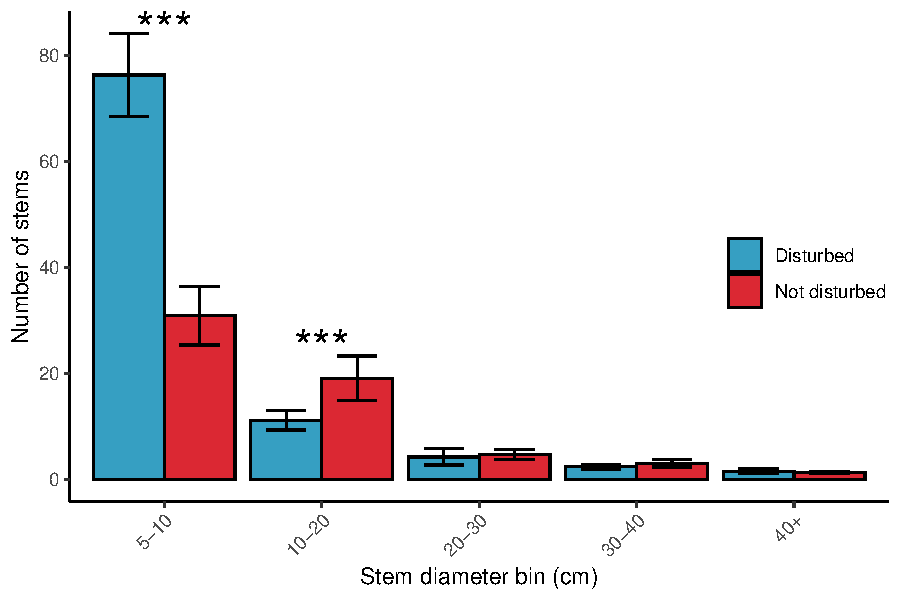
\includegraphics[width=0.8\textwidth]{img/degrad_dbh_bin}
	\caption{Ranked variation between disturbed and undisturbed plots in stem number, with bars according to stem diameter class. Error bars are the mean $\pm$ 1 standard error. Asterisks above pairs of bars refer to the p-values of Poisson general linear models which tested whether disturbed and undisturbed plots differ in the number of stems for different stem diameter classes (***<0.001, **<0.01, *<0.05, .<0.1).}
	\label{degrad_dbh_bin}
\end{figure}

%% If the documentclass option "submit" is chosen, please insert a blank line before and after any math environment (equation and eqnarray environments). This ensures correct linenumbering. The blank line should be removed when the documentclass option is changed to "accept" because the text following an equation should not be a new paragraph. 

%%%%%%%%%%%%%%%%%%%%%%%%%%%%%%%%%%%%%%%%%%
\section{Discussion}

\subsection{Comparison of Bicuar National Park with other woodlands across the miombo ecoregion}

We compared the tree species diversity and woodland structure of arid woodlands in Bicuar National Park in southwest Angola with three other woodland sites across the miombo ecoregion. Our results show that Bicuar National Park is distinct in both woodland structure and species composition from these other woodlands. Notably, plots in Bicuar National Park contained 27 tree species which did not occur at other sites. This lends support for the Hu\'{i}la Plateau as an important area for conservation of southern African woodland landscapes. The woodlands in Bicuar National Park were of low tree basal area, with few large trees except in plots dominated by \textit{Baikiaea plurijuga}. Many other studies have drawn a relationship between water availability and basal area \citep{Terra2018, Strickland2016}, and our study supports this, with Bicuar National Park being the most arid of the four sites considered in our study. The NMDS of species composition also suggests that plots in Bicuar National Park are influenced by aridity. While there are more arid woodlands within southern Africa, with Mopane woodlands for example often being particularly dry, these plots in Bicuar National park represent particularly dry miombo woodlands.

\subsection{Delineation of woodland types within Bicuar National Park}

Within Bicuar National Park, three distinct woodland types were identified. The first, dominated by \textit{Baikiaea plurijuga} and \textit{Baphia massaiensis} represents the Baikiaea woodland type commonly found to the south of the miombo ecoregion \citep{Timberlake2010}. This is supported by \citet{Chisingui2018} who also found Baikiaea woodlands as a distinct woodland type in the Park. \textit{B. plurijuga} has been identified as an important species for conservation, being attractive for selective logging due to its large stature \citep{Ngandwe2017, Wallenfang2015}. The woodlands created by \textit{B. plurijuga} are also an important habitat for elephants (\textit{Loxodonta africana}) \citep{Sianga2017, Mukwashi2012}, with Bicuar National Park and Mupa National Park being key refugia for this animal in the Hu\'{i}la plateau region. The second woodland type, dominated by \textit{Brachystegia tamarindoides} and \textit{Ochna pulchra} represents a form of small stature woodland with a shrubby understorey and sparse canopy trees, which commonly occurs as a result of repeated disturbance by fire, or poor soil structure \citep{Smith2004}. The remaining plots resemble the more archetypical miombo woodland with \textit{Julbernardia paniculata}, though with a number of species not seen in plots further to the east in the miombo ecoregion such as \textit{Strychnos pungens}. This mosaic of woodland types makes Bicuar National Park a valuable reservoir of diversity and strengthens the case for the Park being a key conservation asset within the Hu\'{i}la plateau and the larger southern African region. While there are regional boundaries between Baikiaea and miombo woodlands \citep{White1983}, within Bicuar National Park it is likely that the mosaic of woodland types has been created by a combination of soil water capacity and disturbance history. Bicuar has a distinct landscape of wide shallow grassy valleys surrounded by woodland on higher ground (\autoref{bicuar_map}). On some of these high points the soil is particularly sandy, resembling the Kalahari sand soils found further east and south \citep{Huntley2019}, and these areas coincide with the presence of Baikiaea woodlands \citep{Campbell2002}. High levels of disturbance by fire in these Baikiaea patches may additionally prevent a transition to an alternative woodland type via the control of sapling growth.

\subsection{Comparison of disturbed and undisturbed woodland plots}

Previously disturbed woodlands around the edge of Bicuar National Park were found to share many species with undisturbed plots in the Park, but with some additional species which did not occur in the undisturbed plots. They also lacked notable archetypical miombo species which tend to form larger canopy trees such as \textit{Brachystegia spiciformis} and contained very few \textit{Julbernardia paniculata}, leading to a distinct woodland composition. The species diversity of these disturbed patches was higher on average than was found in the undisturbed plots, a result which has been corroborated by other studies in miombo woodlands \citep{Caro2001, McNicol2018b, Shackleton2000}. Other studies have shown a peak in species richness during woodland regrowth as pioneer species take advantage of a low competition environment, while some later stage woodland species remain as residuals that survived the original disturbance \citep{Goncalves2017, Kalaba2013}. \citet{Goncalves2017} particularly, notes the dominance of \textit{Pericopsis angolensis} and \textit{Combretum} spp. as light-demanding pioneer species, which were found to be abundant in the disturbed plots here. This suggests that reclamation of previously farmed and abandoned land for landscape conservation in this ecological context is a valuable management strategy.

In disturbed plots near the edge of the Park, there was a lack of species which tend to grow to large canopy trees, possibly due to them being repeatedly felled for timber prior to reclamation by the Park, or due to them being unable to recruit into a more open, shrubby woodland. Despite this lack of canopy forming tree species, some disturbed plots had a greater basal area than undisturbed plots, possibly due to high levels of coppicing in these plots or a divergent fire history. Indeed, mean stem density was higher in undisturbed plots. This can lead to species that would otherwise remain small producing a much larger basal area as they grow multiple stems under high disturbance conditions \citep{Luoga2004}. The most common species in the disturbed plots were \textit{Combretum psidioides}, \textit{Combretum collinum} and \textit{Terminalia sericea}, members of the Combretaceae family, all of which more commonly remain as smaller multi-stemmed trees in disturbed woodlands, rather than growing to larger canopy trees \citep{Wyk2014}. This result could be considered at odds with other studies which report lower woody biomass in plots that have experienced harvesting (e.g. \citealt{Muvengwi2020}). It is important to consider however that our study took place in plots that were measured after farming had been abandoned for at least 7 years, with time for regeneration to occur. It is possible that over time tree basal area will decrease as coppiced shrubby trees are replaced by core miombo species in the transition back to miombo woodland \citep{Goncalves2017}. \rnew{Indeed, other studies in miombo woodlands across the ecoregion have reported substantial recovery within seven years, with high levels of biomass accumulation in previously diturbed plots \citep{Chidumayo2013, Goncalves2017}.} Bicuar National Park offers a valuable case study to track woodland regeneration in real-time over the next decade in these previously farmed and now protected woodland plots, which could improve our understanding of this potential post-disturbance peak in basal area.

In conclusion, the woodlands of Bicuar National Park represent an important woodland refuge at the far western extent of the miombo ecoregion. These woodlands, both those disturbed by previous farming activity and those which remain undisturbed, possess a number of species not found commonly in other miombo woodland plots around the region. They may also house important genetic variation for widespread species, representing populations adapted to more arid conditions. Our study highlights the variation in species composition across the miombo ecoregion and underlines the need for studies which incorporate plot data from multiple locations to reach generalisable conclusions about the region as a whole. Additionally, the installation of 15 one hectare woodland monitoring plots and a further twenty 20x50 m plots in previously farmed and now protected land offer a valuable natural laboratory to further explore the dynamics of dry miombo woodlands of the Hu\'{i}la plateau. Bicuar National Park should be considered a key conservation asset within the Hu\'{i}la plateau and within the miombo ecoregion as a whole, as a successfully protected example of an arid woodland mosaic.

%\section{Conclusions}

%This section is not mandatory, but can be added to the manuscript if the discussion is unusually long or complex.

%\section{Patents}
%This section is not mandatory, but may be added if there are patents resulting from the work reported in this manuscript.

%%%%%%%%%%%%%%%%%%%%%%%%%%%%%%%%%%%%%%%%%%
\vspace{6pt} 

%%%%%%%%%%%%%%%%%%%%%%%%%%%%%%%%%%%%%%%%%%
%% optional
%\supplementary{The following are available online at \linksupplementary{s1}, Figure S1: title, Table S1: title, Video S1: title.}

% Only for the journal Methods and Protocols:
% If you wish to submit a video article, please do so with any other supplementary material.
% \supplementary{The following are available at \linksupplementary{s1}, Figure S1: title, Table S1: title, Video S1: title. A supporting video article is available at doi: link.}

%%%%%%%%%%%%%%%%%%%%%%%%%%%%%%%%%%%%%%%%%%
\authorcontributions{Investigation and project administration was conducted by J.L.G., F.M.G., J.J.T. and A.V.T. (Bicuar National Park), C.M.R. (Tanzania, Mozambique), J.I.M. and M.N.S. (DRC). The study was conceived by J.L.G. and K.G.D.. Data curation, methodology, formal analysis and writing--original draft preparation was conducted by J.L.G.. All authors contributed to writing--review and editing.}

%For research articles with several authors, a short paragraph specifying their individual contributions must be provided. The following statements should be used ``conceptualization, X.X. and Y.Y.; methodology, X.X.; software, X.X.; validation, X.X., Y.Y. and Z.Z.; formal analysis, X.X.; investigation, X.X.; resources, X.X.; data curation, X.X.; writing--original draft preparation, X.X.; writing--review and editing, X.X.; visualization, X.X.; supervision, X.X.; project administration, X.X.; funding acquisition, Y.Y.'', please turn to the  \href{http://img.mdpi.org/data/contributor-role-instruction.pdf}{CRediT taxonomy} for the term explanation. Authorship must be limited to those who have contributed substantially to the work reported.
%%%%%%%%%%%%%%%%%%%%%%%%%%%%%%%%%%%%%%%%%%
\funding{Final data preparation across all sites was funded by SEOSAW (a Socio-Ecological Observatory for the Southern African Woodlands), a NERC-funded project (Grant No. NE/P008755/1). The installation of woodland plots in Bicuar National Park and their data collection was funded by the National Geographic Society (Grant No. EC-51464R-18) to FMG, AVC, KGD and JLG. JLG was supported by a NERC E3 Doctoral Training Programme PhD studentship (Grant No. NE/L002558/1). The APC was funded by the University of Edinburgh.}
% APC = Article processing charge

%%%%%%%%%%%%%%%%%%%%%%%%%%%%%%%%%%%%%%%%%%
\acknowledgments{The rangers at Bicuar National Park are gratefully acknowledged for their help in installing the woodland survey plots and for their help with numerous other incidental challenges during fieldwork. Domingos Fortunato P. F\'{e}lix da Silva, Abel C. E. Cahali, Felisberto Gomes Armando, Jos\'{e} Cam\^{o}ngua Lu\'{i}s, Manuel Jundo Cachissapa and Henrique Jacinto are acknowledged for their help in conducting plot measurements in Bicuar National Park.}

%%%%%%%%%%%%%%%%%%%%%%%%%%%%%%%%%%%%%%%%%%
\conflictsofinterest{The authors declare no conflict of interest. The funders had no role in the design of the study; in the collection, analyses, or interpretation of data; in the writing of the manuscript, or in the decision to publish the results.} 

%%%%%%%%%%%%%%%%%%%%%%%%%%%%%%%%%%%%%%%%%%
%% optional
\abbreviations{The following abbreviations are used in this manuscript:\\

\noindent 
\begin{tabular}{@{}ll}
	ANOVA & Analysis of Variance\\
	DD & Decimal Degrees\\
	MAP & Mean Annual Precipitation\\
	MAT & Mean Annual Temperature\\
	MAT SD & Standard Deviation of Mean Annual Temperature (Seasonality)\\
	NMDS & Non-metric Multidimensional Scaling\\
	NP & National Park\\
\end{tabular}}

\newpage{} 

%%%%%%%%%%%%%%%%%%%%%%%%%%%%%%%%%%%%%%%%%%
%% optional
\appendixtitles{yes} %Leave argument "no" if all appendix headings stay EMPTY (then no dot is printed after "Appendix A"). If the appendix sections contain a heading then change the argument to "yes".
\appendix

\section{Estimation of stem diameter at 1.3 m via tree taper} \label{appendixa}

\begin{lstlisting}[language=R]
##' @author Casey M. Ryan
##' @return d130, the estimated diameter at a POM of 1.3 m (in cm). 
##' @param d_in the diameter measured at the POM (in cm)
##' @param POM the height of the POM (in m)
##' @details The adjustment based on tree taper model developed as part of 
##'   the ACES project (Abrupt Changes in Ecosystem Services 
##'   https://miomboaces.wordpress.com/), using data from the miombo of Niassa. 
##'   The model is a cubic polynomial, with three equations for different sized stems. 
##' @section Warning: POMs >1.7 m are not adjusted.
POMadj <- function(d_in, POM) {
  stopifnot(is.numeric(d_in),
    is.numeric(POM),
    POM >= 0,
    sum(is.na(POM))==0,
    length(POM) == length(d_in))
  if (any(POM > 1.7))
    warning("POMs >1.7 m are outside the calibration data, no correction applied") 
  NAS <- is.na(d_in)
  d_in_clean <- d_in[!NAS]
  POM_clean <- POM[!NAS]
  # define the size class edges:
  edges <- c(5.0, 15.8, 26.6, 37.4)
  sm <- d_in_clean < edges[2]
  med <- d_in_clean >= edges[2] & d_in_clean < edges[3]
  lg <- d_in_clean >= edges[3]
  
  # compute predictions for delta_d, for all size classes
  delta_d <- data.frame(
    # if small:
    small =  3.4678+-5.2428 * 
   	  POM_clean + 2.9401 * 
      POM_clean^2+-0.7141 * 
      POM_clean^3,
    # if med
    med =  4.918+-8.819 * 
      POM_clean + 6.367 * 
      POM_clean^2+-1.871 * 
      POM_clean^3,
    # if large
    large =  9.474+-18.257 * 
      POM_clean + 12.873 * 
      POM_clean^2+-3.325 * 
      POM_clean^3
  )
  # index into the right size class
  dd <- NA_real_
  dd[sm] <- delta_d$small[sm]
  dd[med] <- delta_d$med[med]
  dd[lg] <- delta_d$large[lg]
  dd[POM_clean > 1.7] <- 0  # to avoid extrapolation mess
  
  # add NAs back in
  d130 <- NA
  d130[NAS] <- NA
  d130[!NAS] <- d_in_clean - dd
  
  if (any(d130[!NAS] < 0))
    warning("Negative d130 estimated, replaced with NA")
  d130[d130 <= 0 & !is.na(d130)] <- NA
  return(d130)
}
\end{lstlisting}

% The appendix is an optional section that can contain details and data supplemental to the main text. For example, explanations of experimental details that would disrupt the flow of the main text, but nonetheless remain crucial to understanding and reproducing the research shown; figures of replicates for experiments of which representative data is shown in the main text can be added here if brief, or as Supplementary data. Mathematical proofs of results not central to the paper can be added as an appendix.
% All appendix sections must be cited in the main text. In the appendixes, Figures, Tables, etc. should be labeled starting with `A', e.g., Figure A1, Figure A2, etc. 

%%%%%%%%%%%%%%%%%%%%%%%%%%%%%%%%%%%%%%%%%%
\reftitle{References}

% Please provide either the correct journal abbreviation (e.g. according to the “List of Title Word Abbreviations” http://www.issn.org/services/online-services/access-to-the-ltwa/) or the full name of the journal.
% Citations and References in Supplementary files are permitted provided that they also appear in the reference list here. 

%=====================================
% References, variant A: external bibliography
%=====================================
\externalbibliography{yes}
\bibliography{lib}

% To cite two works by the same author: \citeauthor{ref-journal-1a} (\citeyear{ref-journal-1a}, \citeyear{ref-journal-1b}). This produces: Whittaker (1967, 1975)
% To cite two works by the same author with specific pages: \citeauthor{ref-journal-3a} (\citeyear{ref-journal-3a}, p. 328; \citeyear{ref-journal-3b}, p.475). This produces: Wong (1999, p. 328; 2000, p. 475)

\end{document}

